\documentclass{standalone}
\usepackage{tikz}
\usetikzlibrary{positioning,fit,matrix}
\usepackage{todonotes}
%\usepackage{scalefnt}

%\tikzset{%
%  textnode/.style     = {\sffamily font=\fontsize{10}{12.4}\selectfont},
%}

\begin{document}

\sffamily%\sansmath
%\scalefont{0.01}
%\fontsize{8}{10.0}\selectfont

\begin{tikzpicture}


%%%%% L1 %%%%%

% A
\node[inner sep=0] (A1) {
\includegraphics[width=2cm]{3DFamilies/A/1618470405_25d.png}};
\node[inner sep=0, right=0mm of A1] (A2) {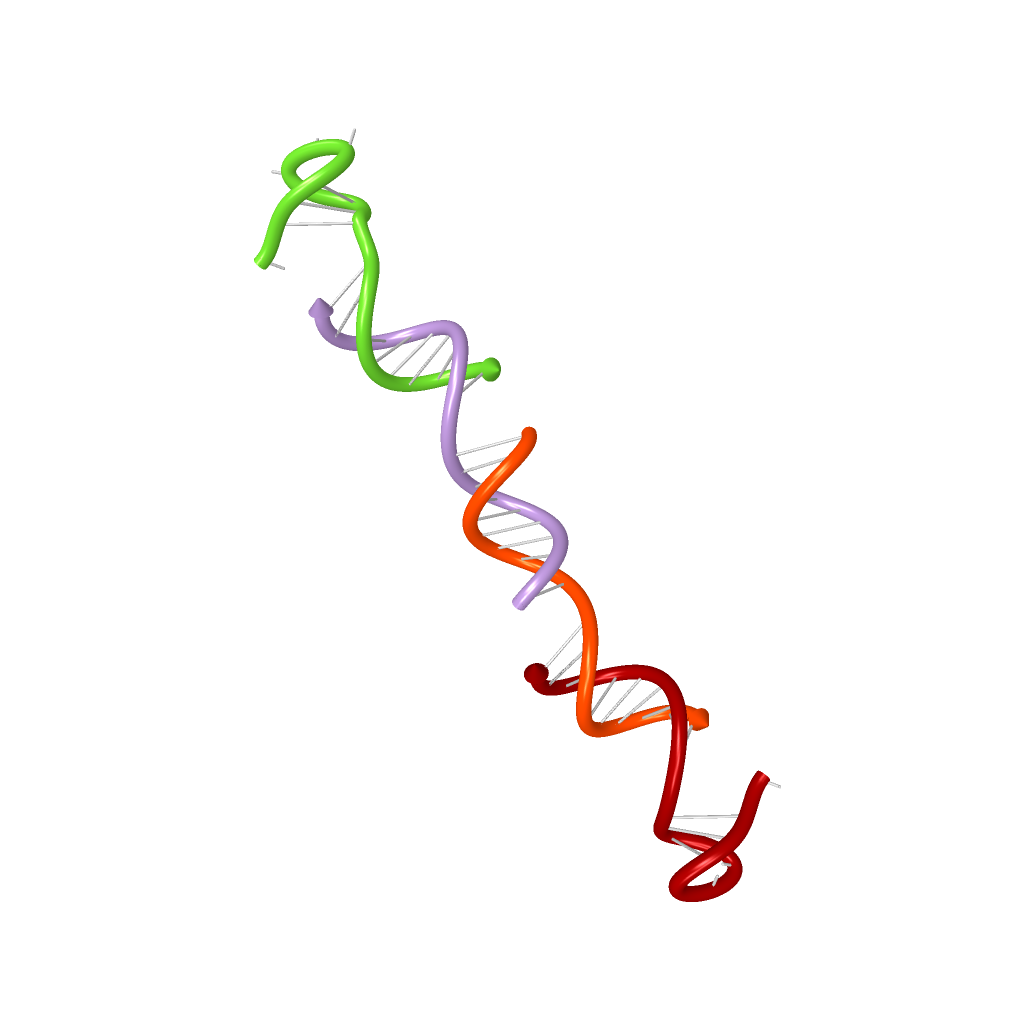
\includegraphics[width=2cm]{3DFamilies/A/1618470409_25d.png}};
\node[inner sep=0, right=0mm of A2] (A3) {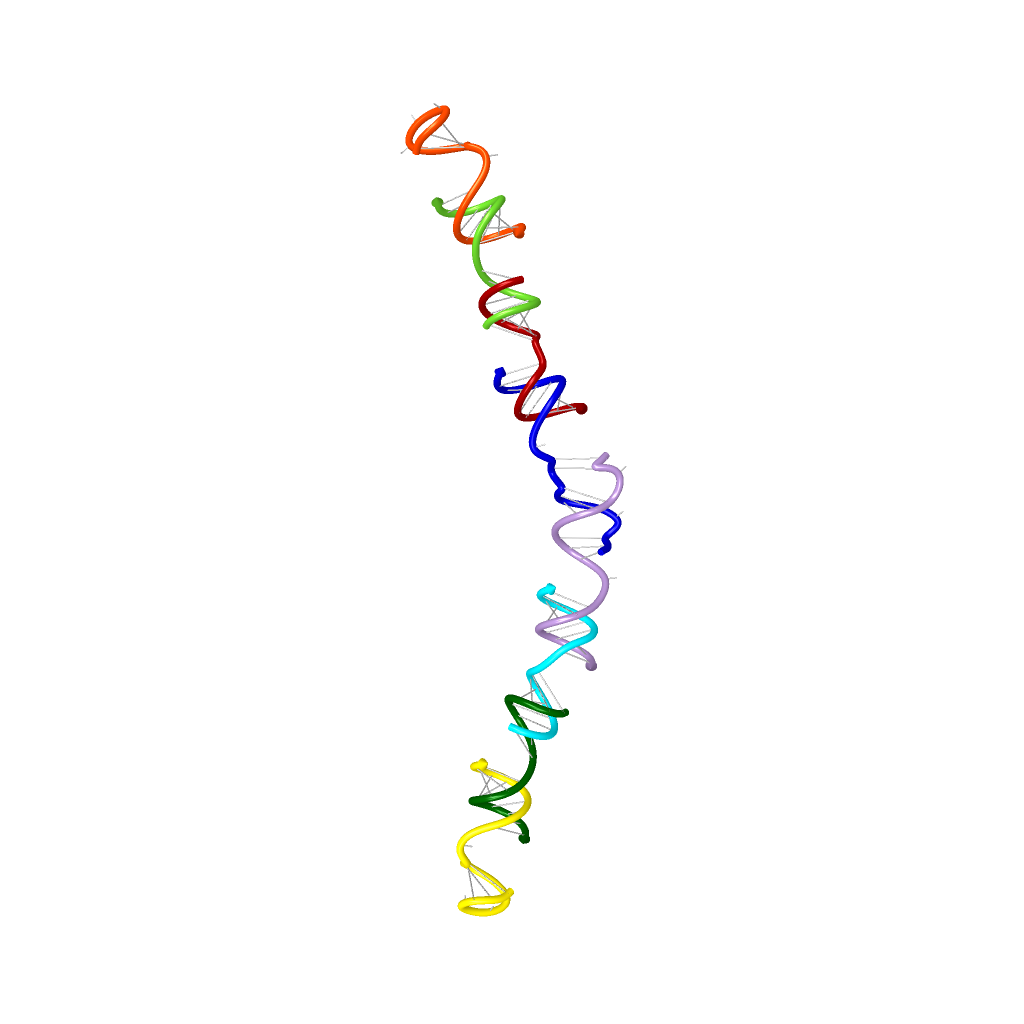
\includegraphics[width=2cm]{3d/L1-A_random.png}};

% B
\node[inner sep=0, right=10mm of A3] (B1) {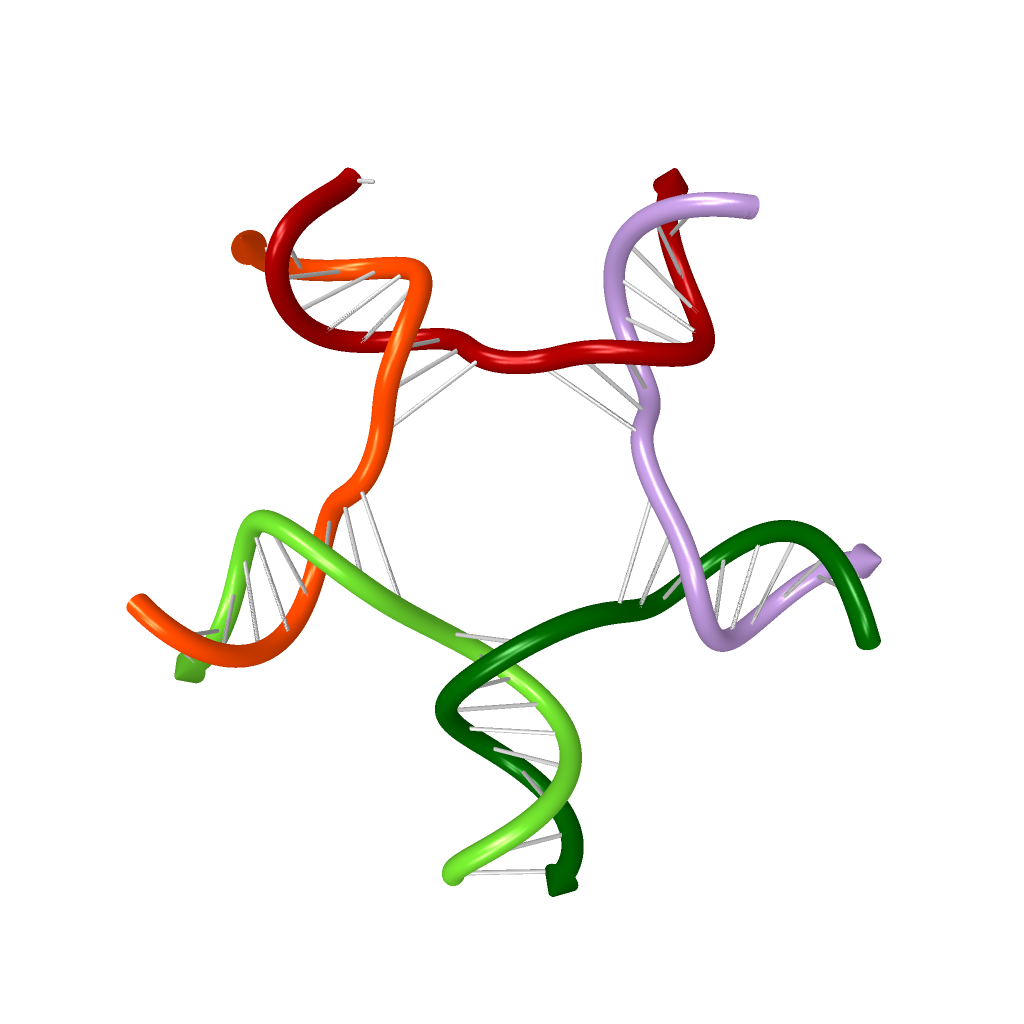
\includegraphics[width=2cm]{3DFamilies/B/1618470983_25d.png}};
\node[inner sep=0, right=0mm of B1] (B2) {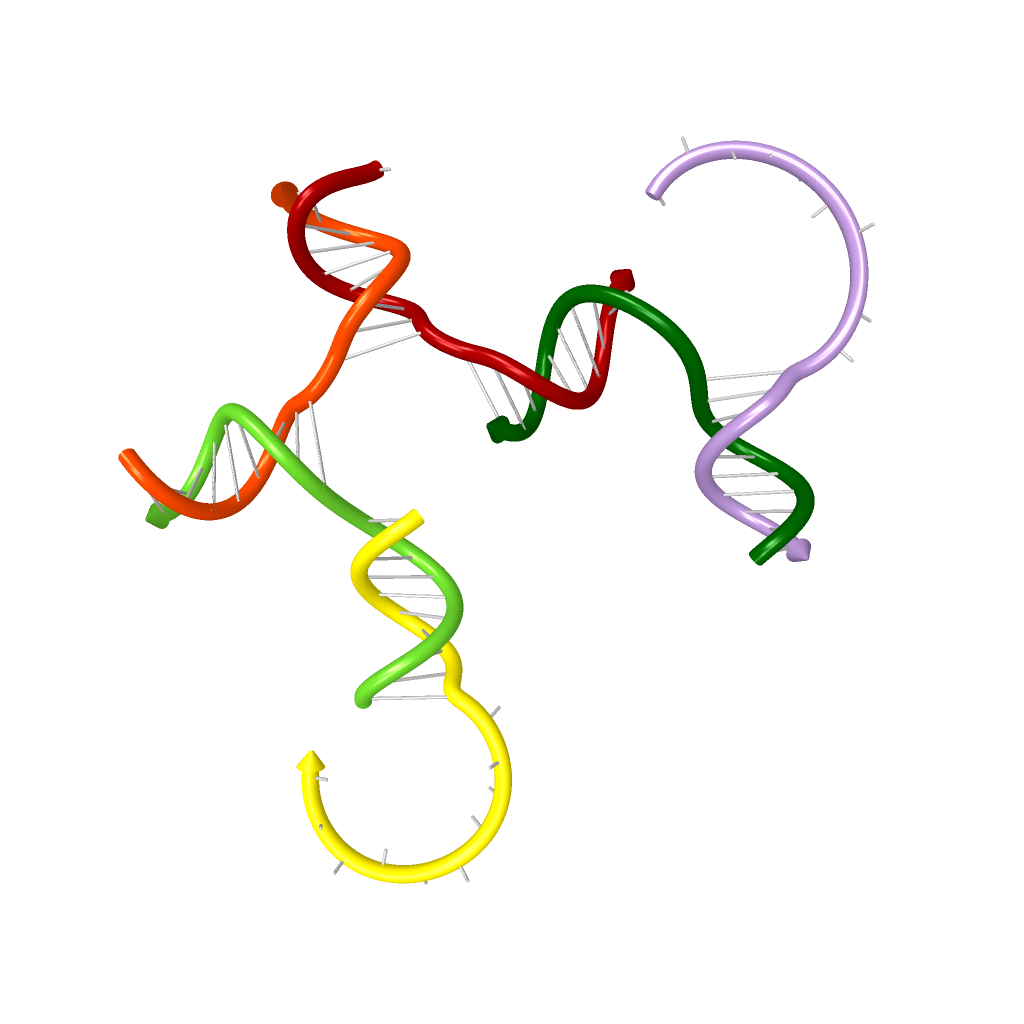
\includegraphics[width=2cm]{3DFamilies/B/1618471349_25d.png}};
\node[inner sep=0, right=0mm of B2] (B3) {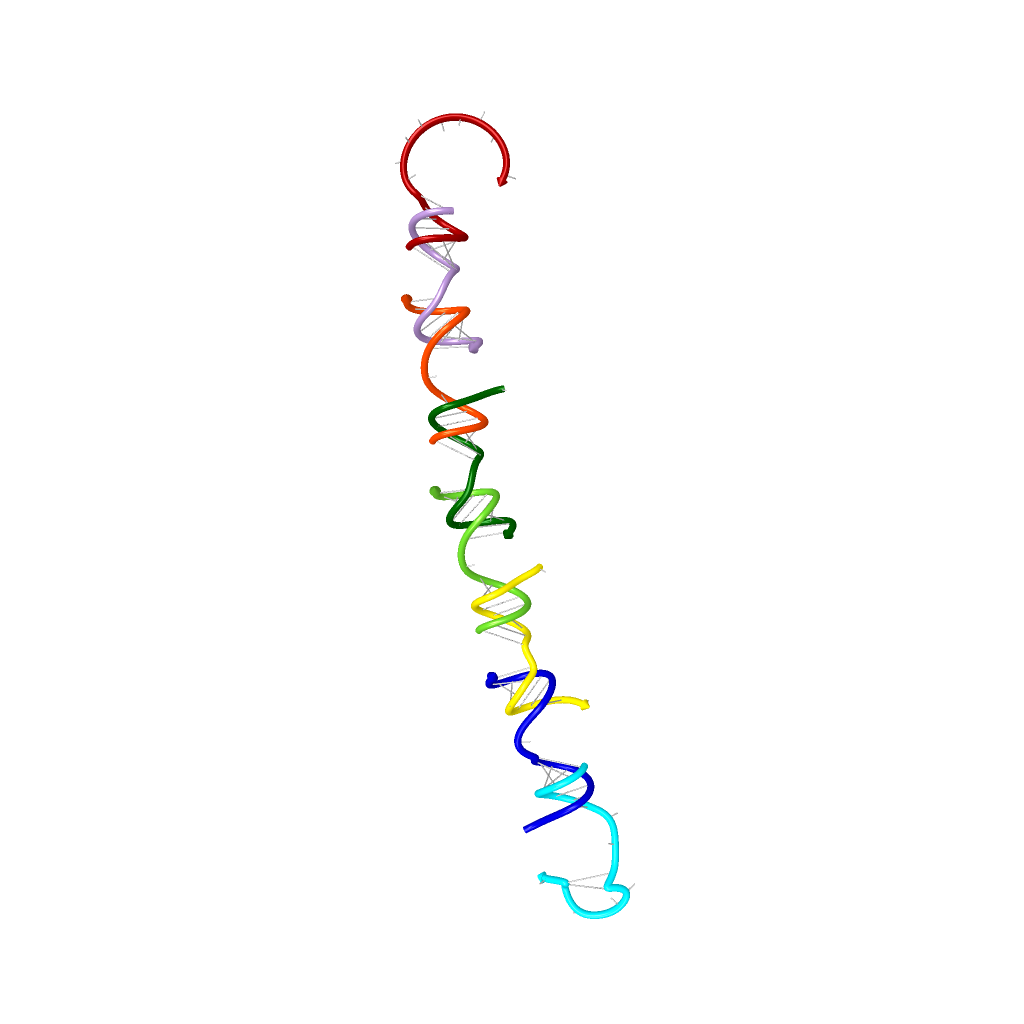
\includegraphics[width=2cm]{3d/L1-B_random.png}};

% C
\node[inner sep=0, below=0mm of A1] (C1) {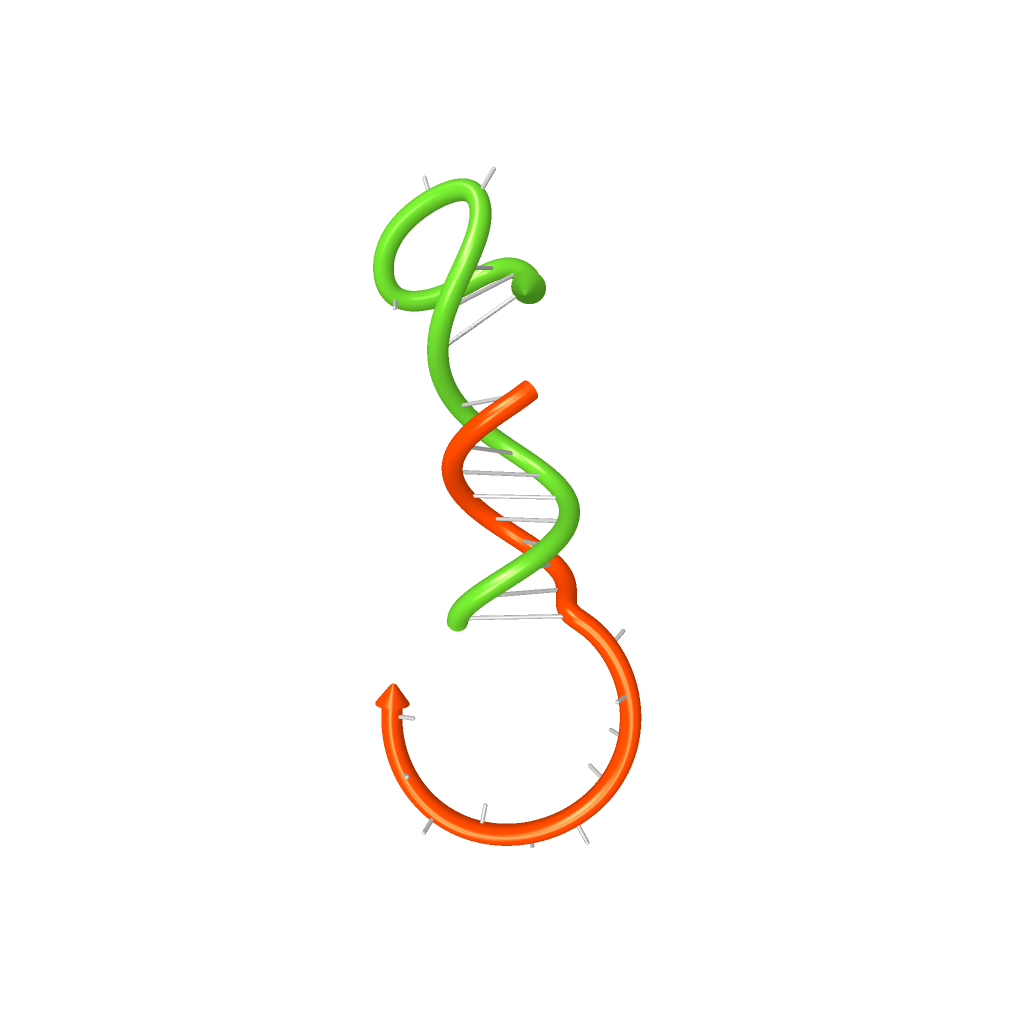
\includegraphics[width=2cm]{3DFamilies/C/1618534354_25d.png}};
\node[inner sep=0, right=0mm of C1] (C2) {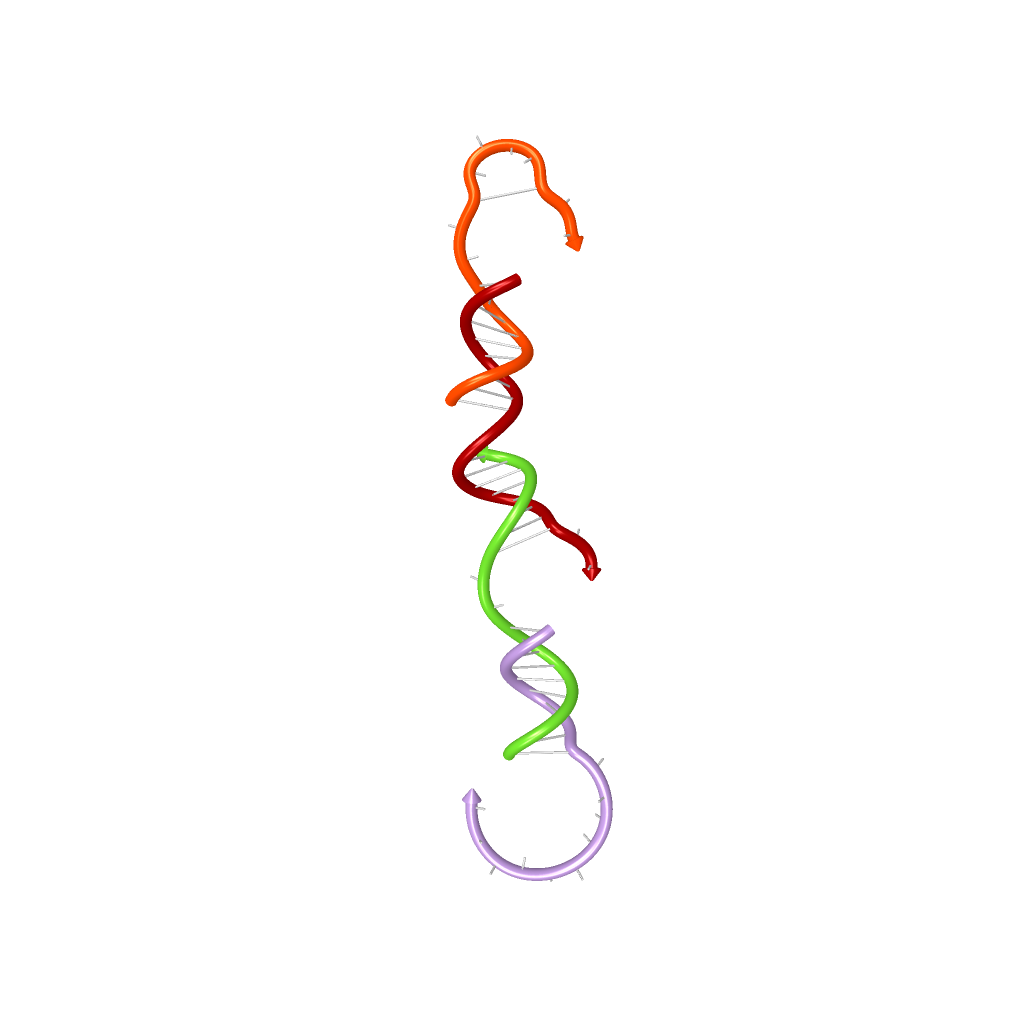
\includegraphics[width=2cm]{3DFamilies/C/1618534385_25d.png}};
\node[inner sep=0, right=0mm of C2] (C3) {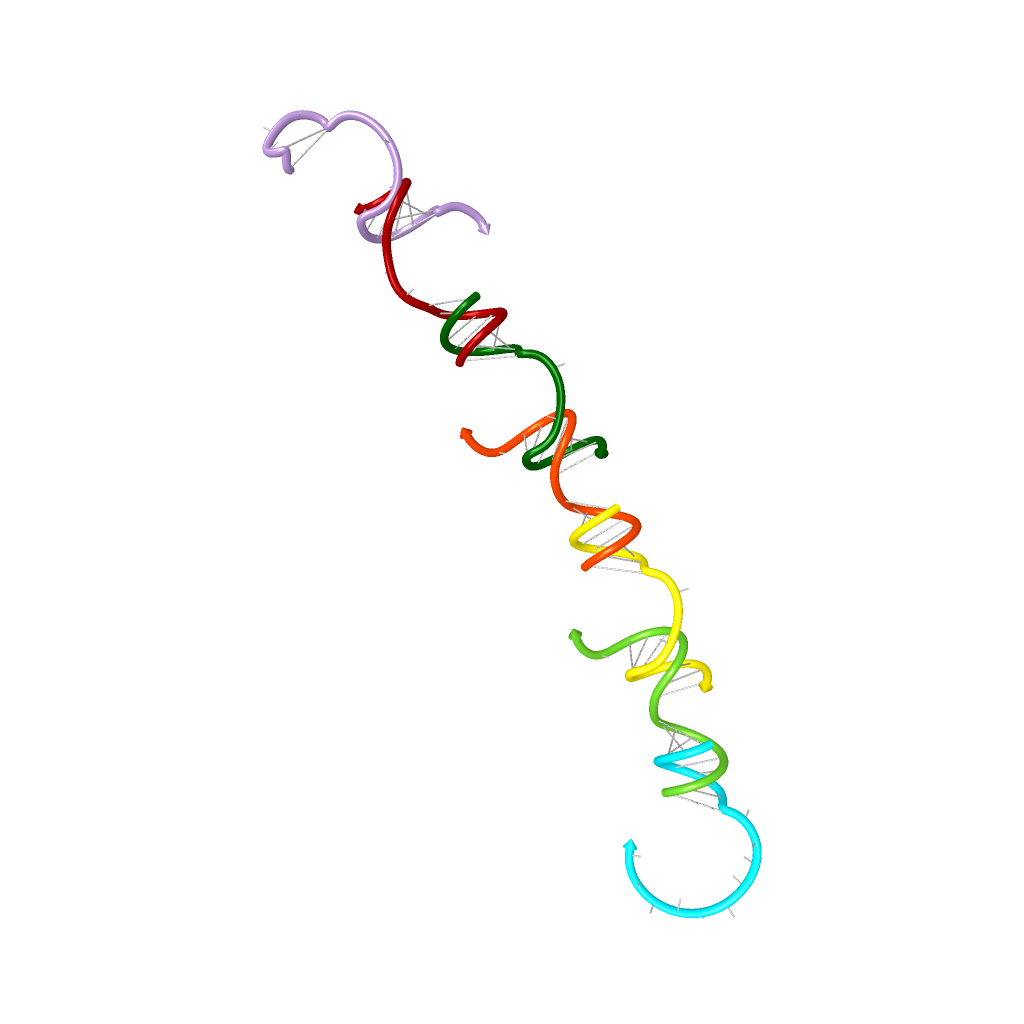
\includegraphics[width=2cm]{3d/L1-C_random.png}};

% D
\node[inner sep=0, right=10mm of C3] (D1) {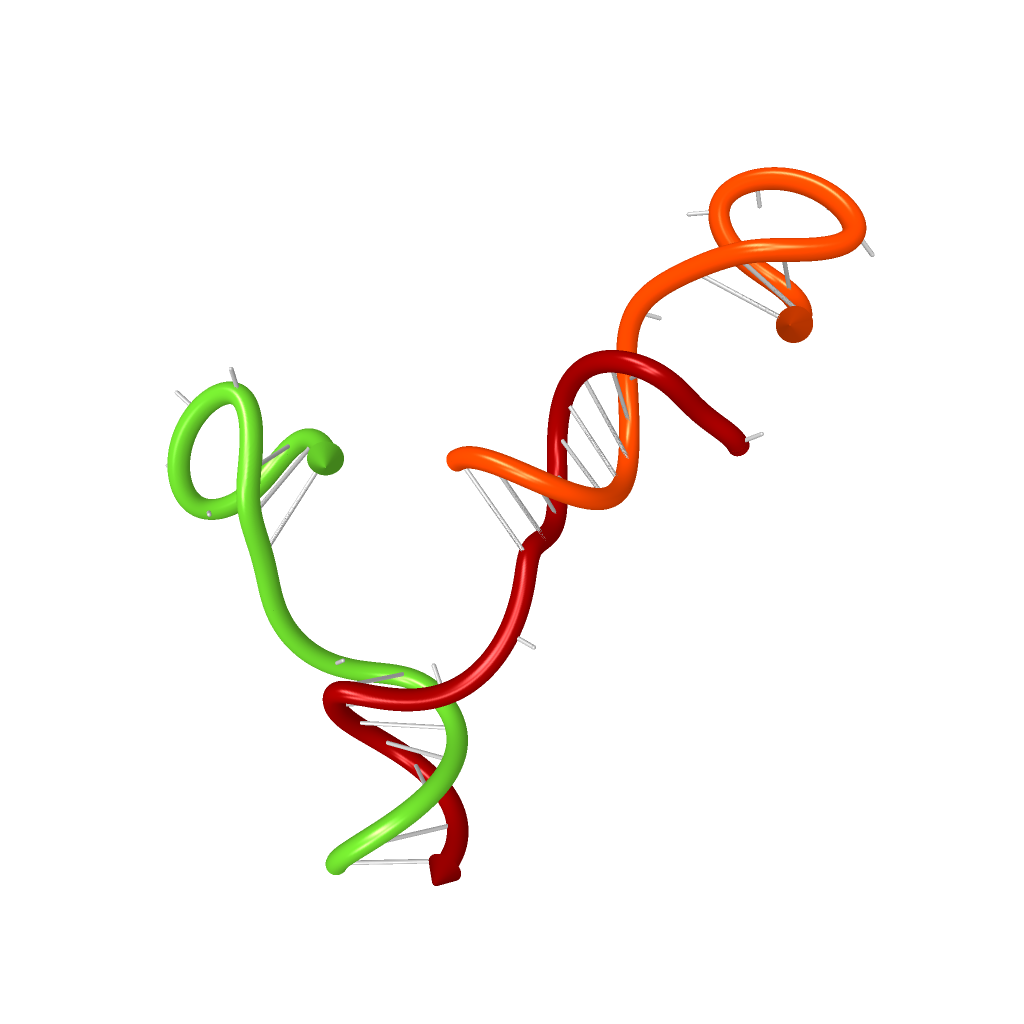
\includegraphics[width=2cm]{3DFamilies/D/1618535459_25d.png}};
\node[inner sep=0, right=0mm of D1] (D2) {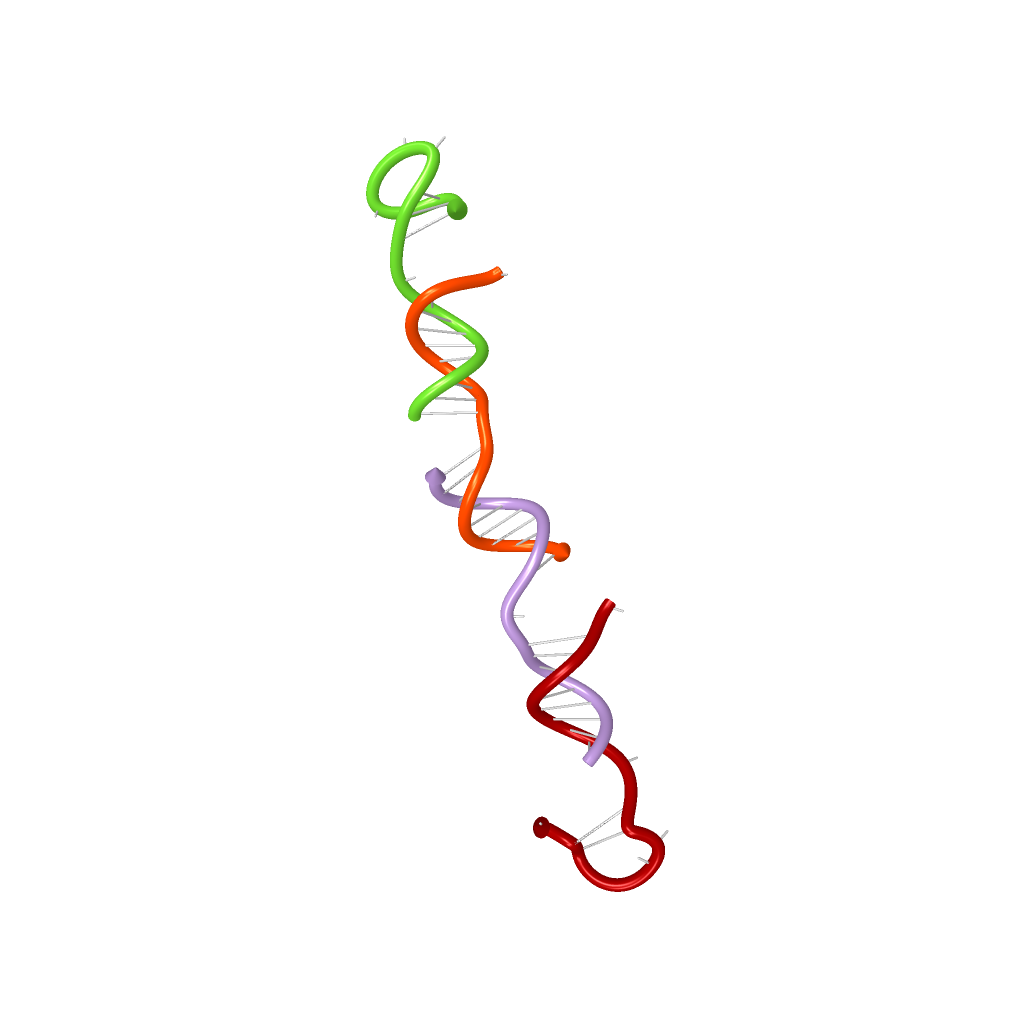
\includegraphics[width=2cm]{3DFamilies/D/1618535695_25d.png}};
\node[inner sep=0, right=0mm of D2] (D3) {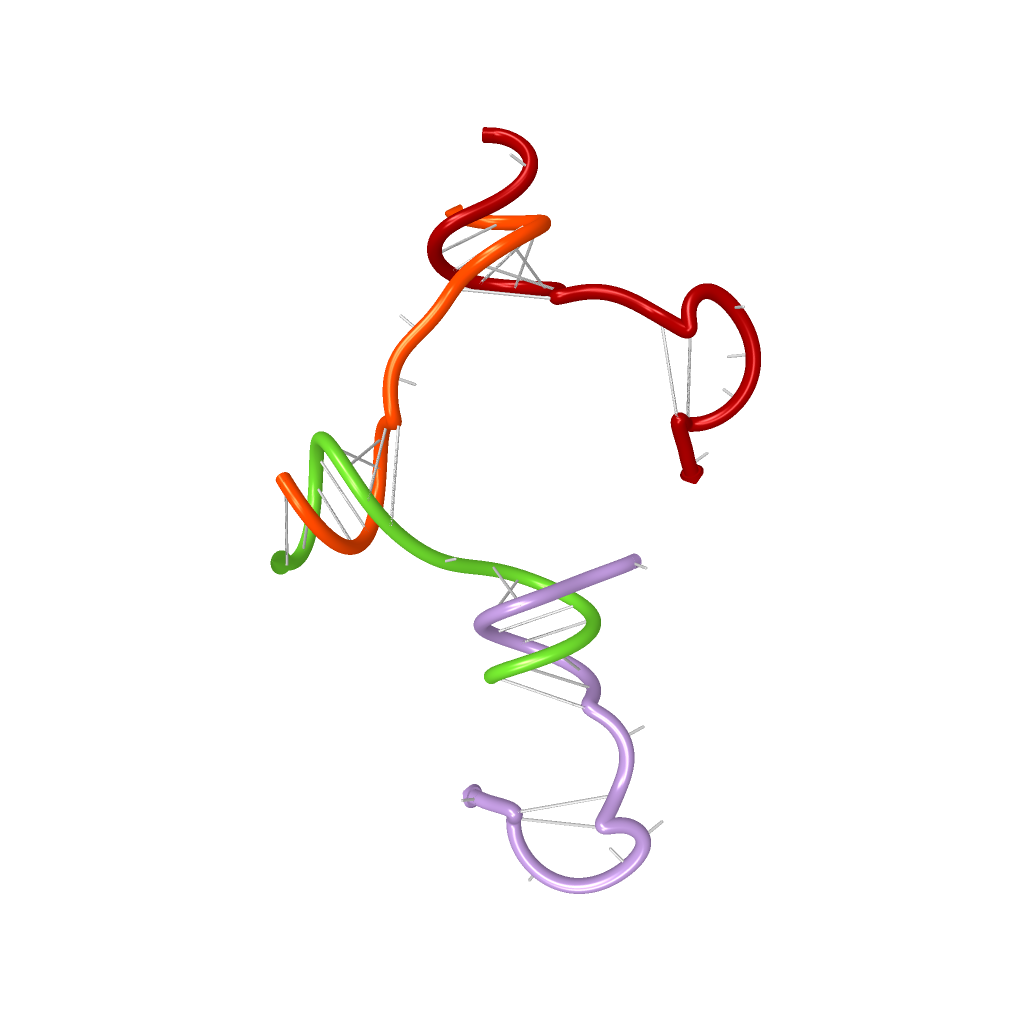
\includegraphics[width=2cm]{3d/L1-D_random.png}};


%%%%% L2 %%%%%

% E
\node[inner sep=0, below=5mm of C1] (E1) {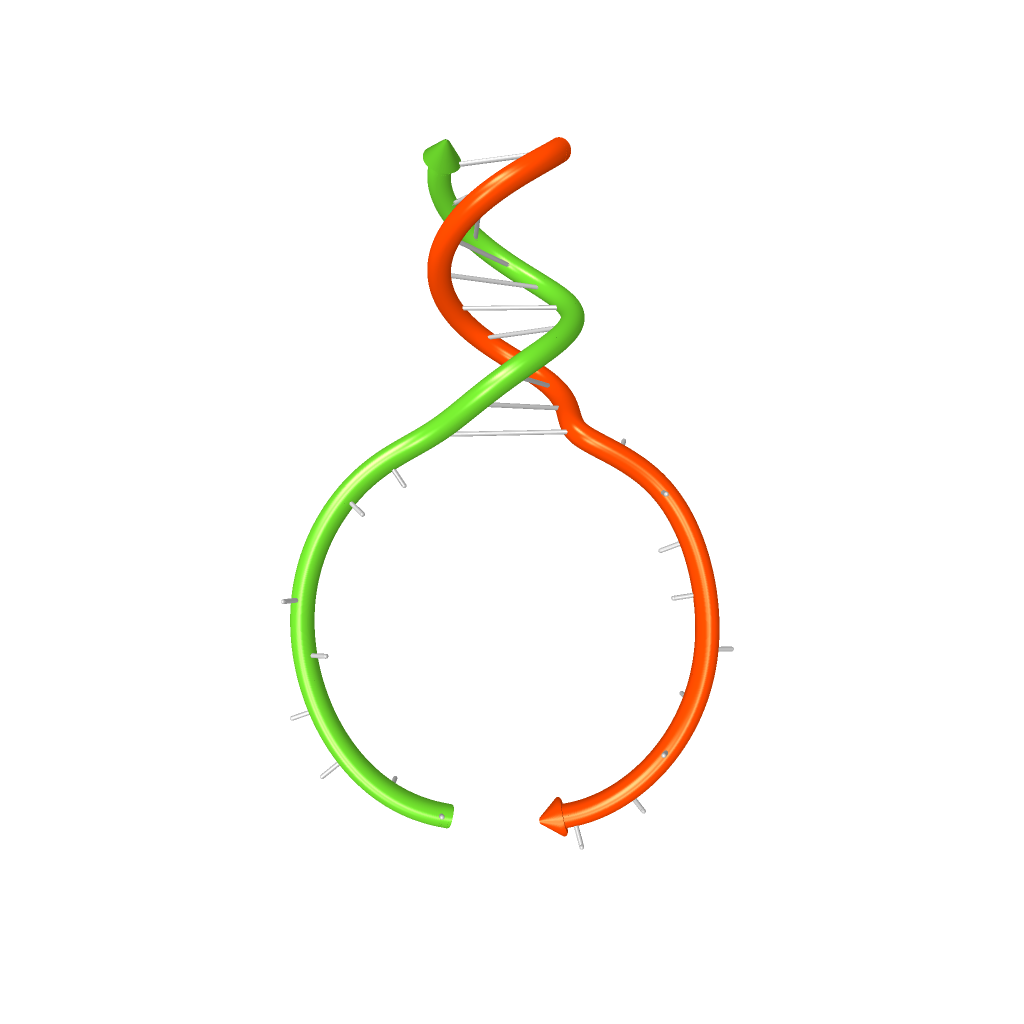
\includegraphics[width=2cm]{3DFamilies/E/1618554219_25d.png}};
\node[inner sep=0, right=0mm of E1] (E2) {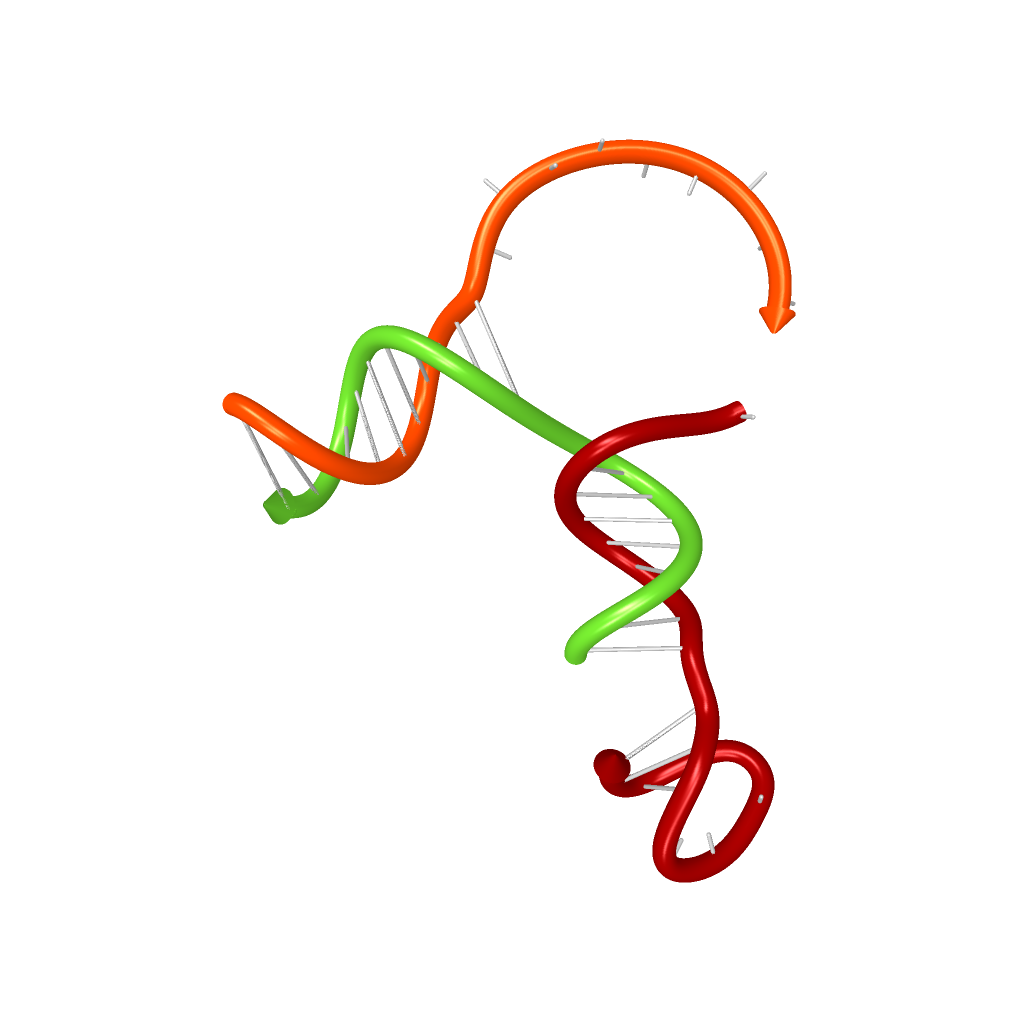
\includegraphics[width=2cm]{3DFamilies/E/1618554258_25d.png}};
\node[inner sep=0, right=0mm of E2] (E3) {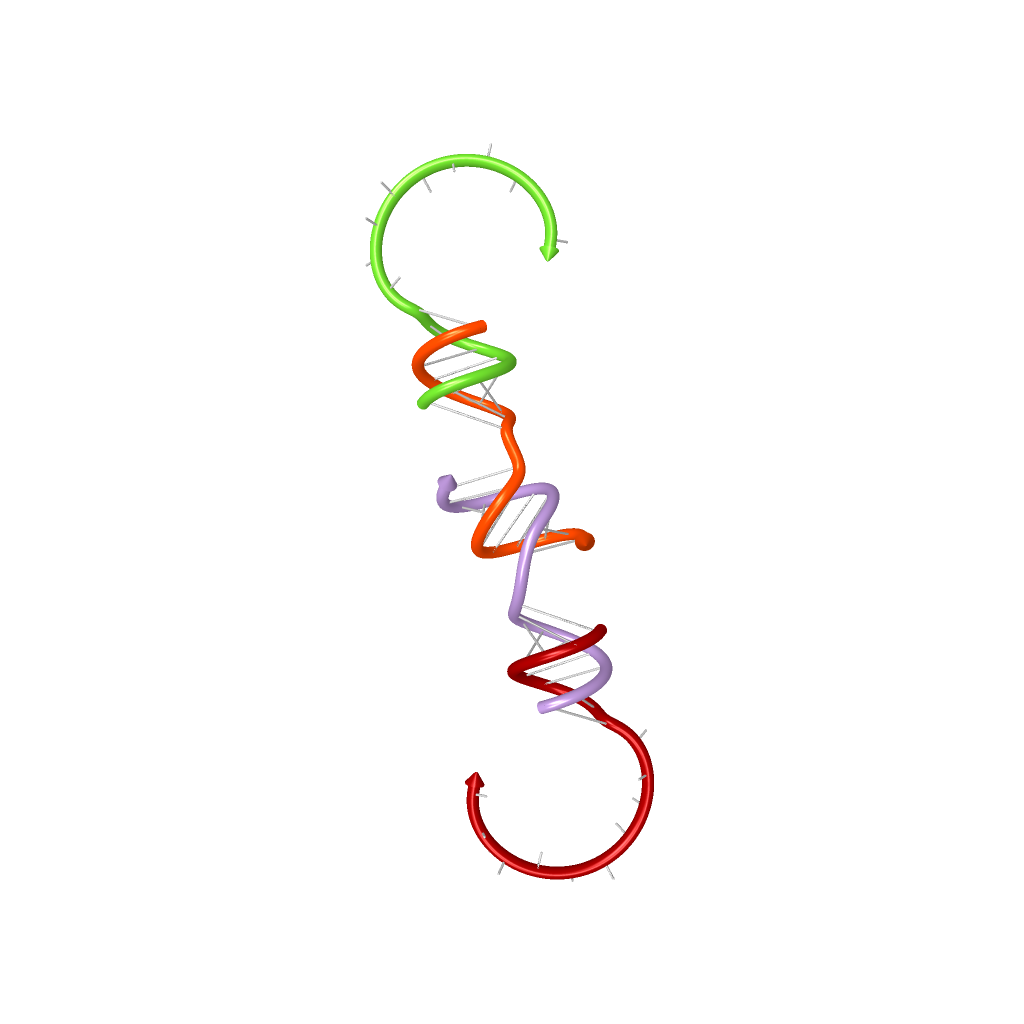
\includegraphics[width=2cm]{3d/L2-E_random.png}};

% F
\node[inner sep=0, right=10mm of E3] (F1) {
\includegraphics[width=2cm]{3DFamilies/F/1618554945_25d.png}};
\node[inner sep=0, right=0mm of F1] (F2) {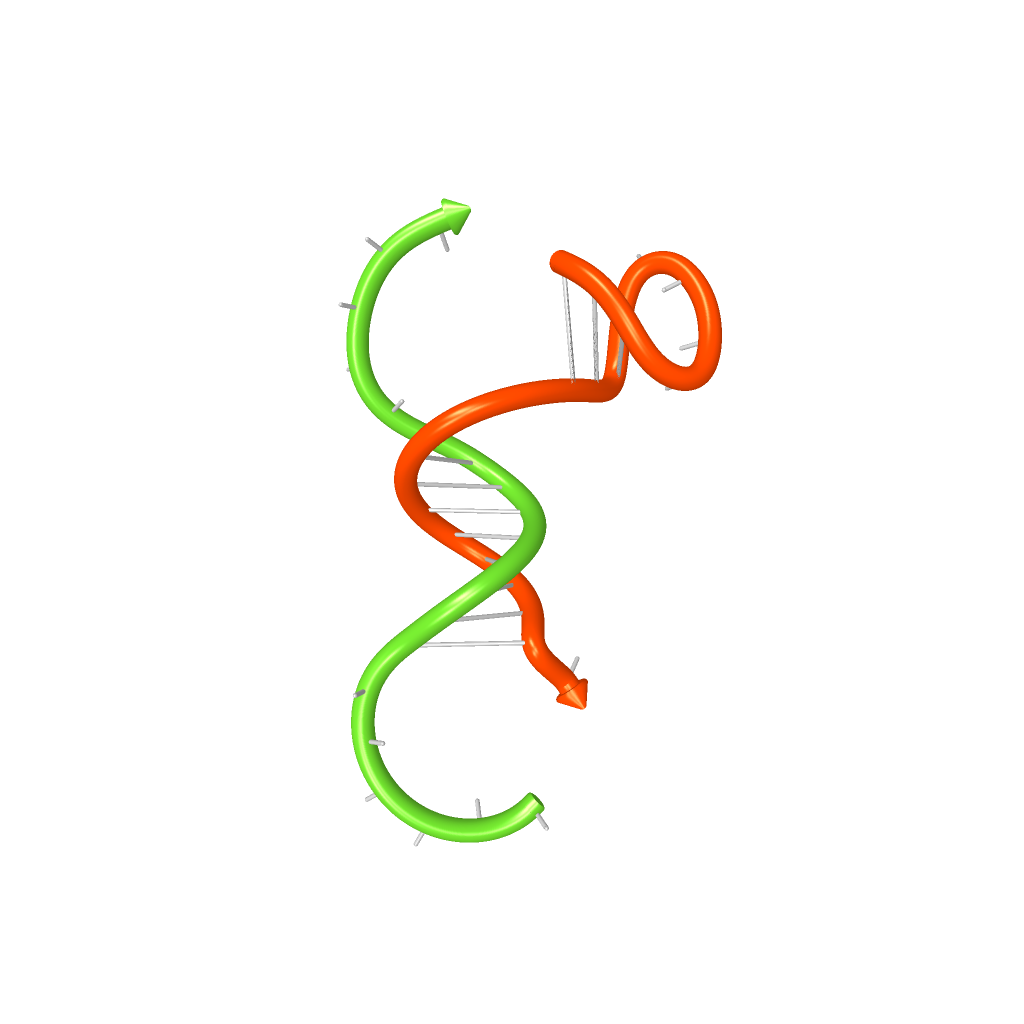
\includegraphics[width=2cm]{3DFamilies/F/1618554954_25d.png}};
\node[inner sep=0, right=0mm of F2] (F3) {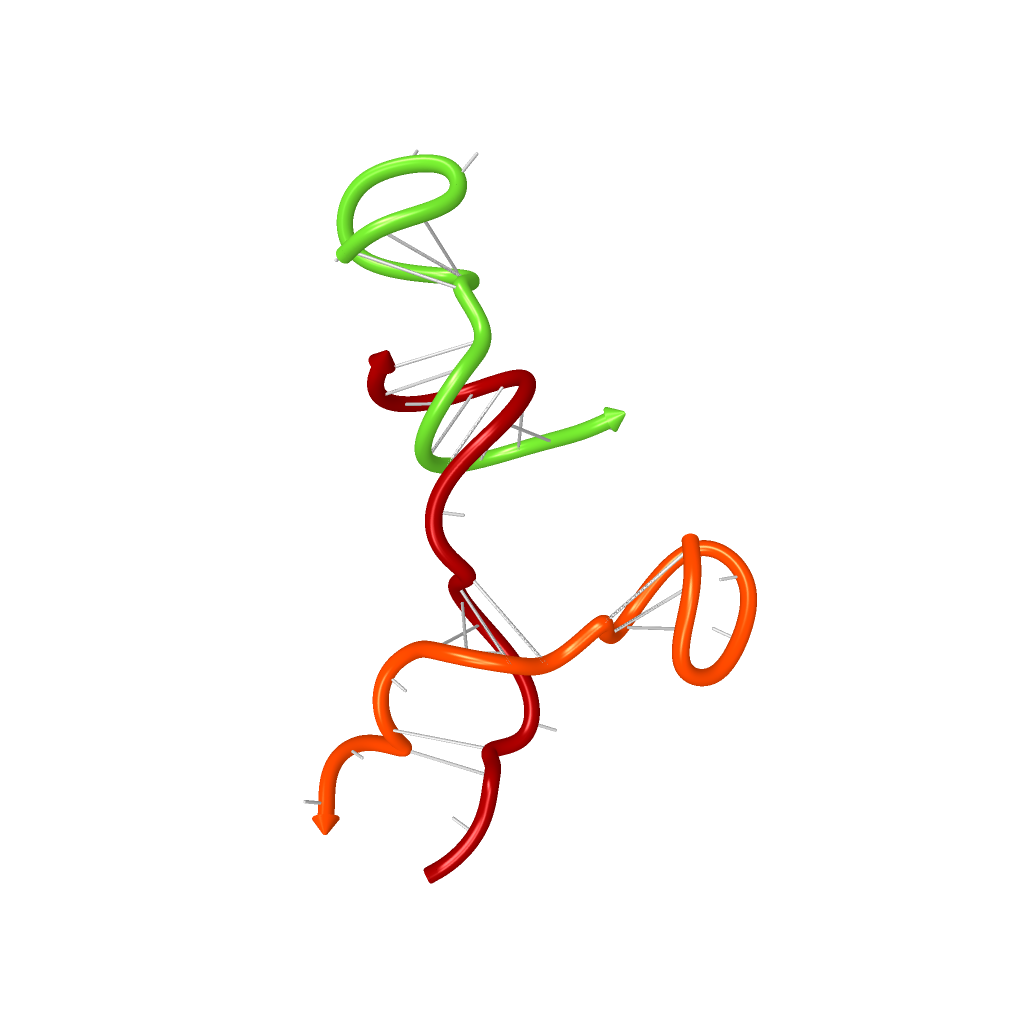
\includegraphics[width=2cm]{3d/L2-F_GA.png}};

% G
\node[inner sep=0, below=0mm of E1] (G1) {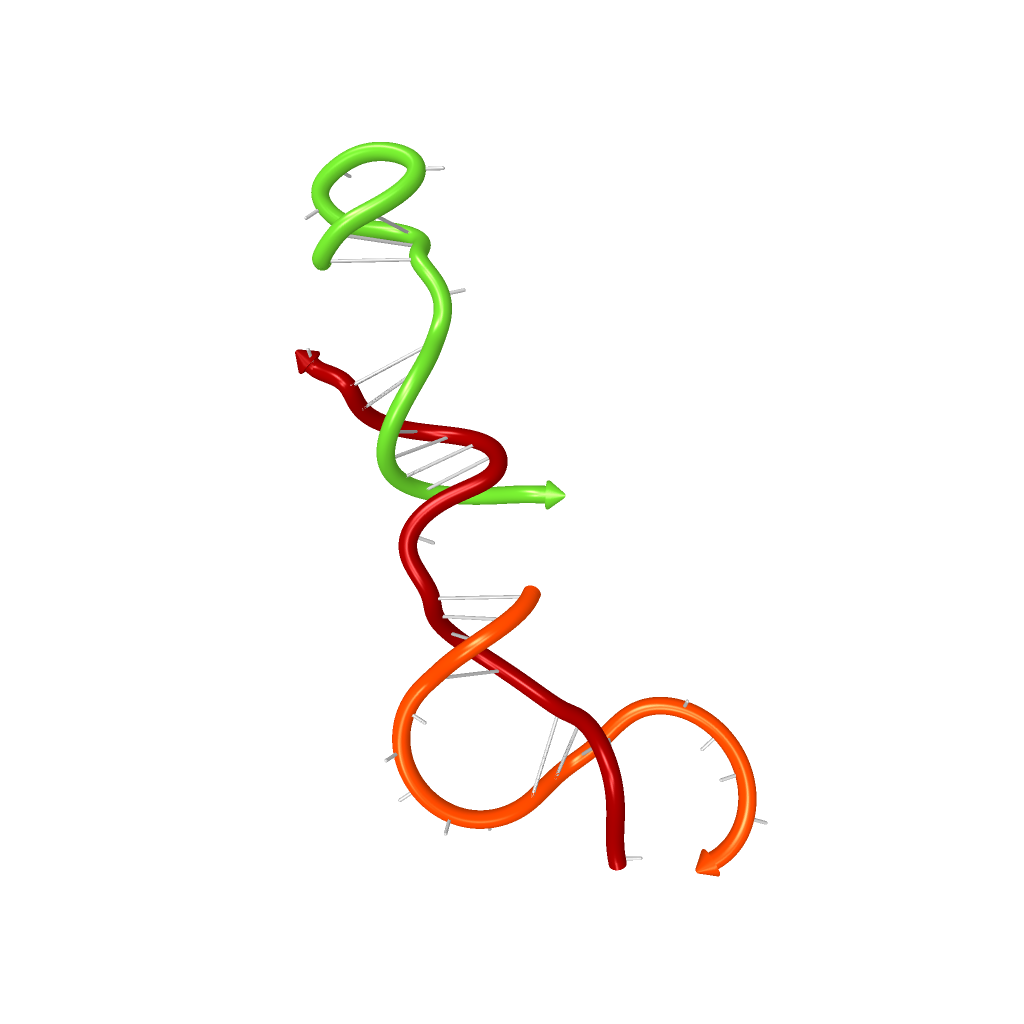
\includegraphics[width=2cm]{3DFamilies/G/1618555112_25d.png}};
\node[inner sep=0, right=0mm of G1] (G2) {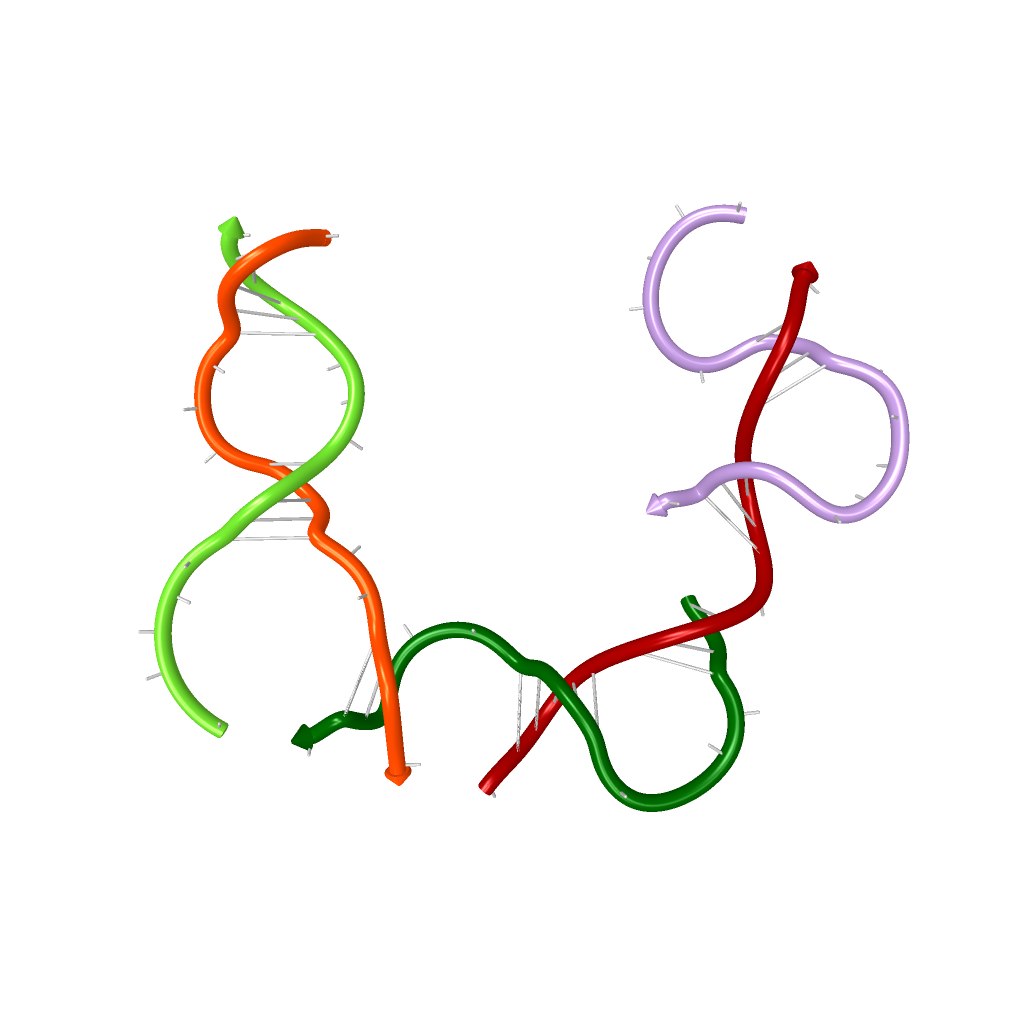
\includegraphics[width=2cm]{3DFamilies/G/1618555157_25d.png}};
\node[inner sep=0, right=0mm of G2] (G3) {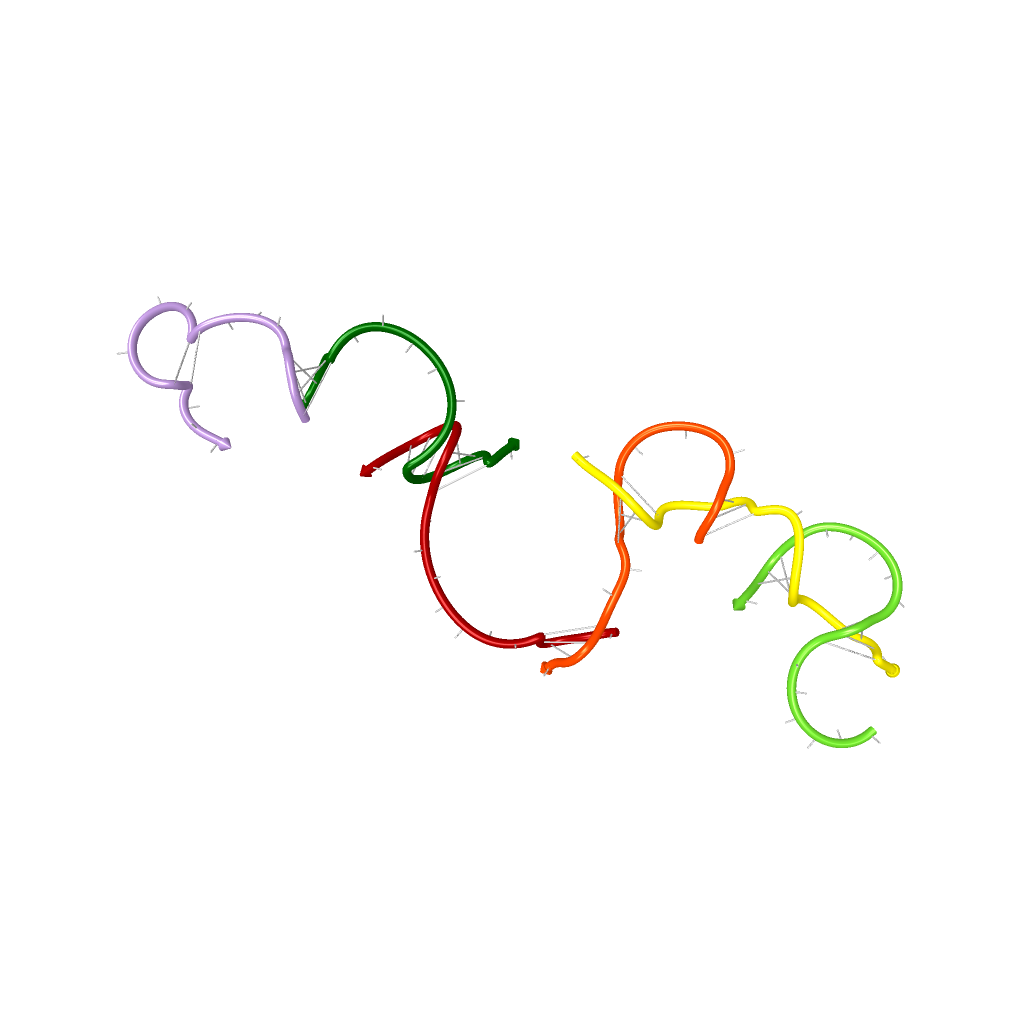
\includegraphics[width=2cm]{3d/L2-G_GA.png}};

% H
\node[inner sep=0, right=10mm of G3] (H1) {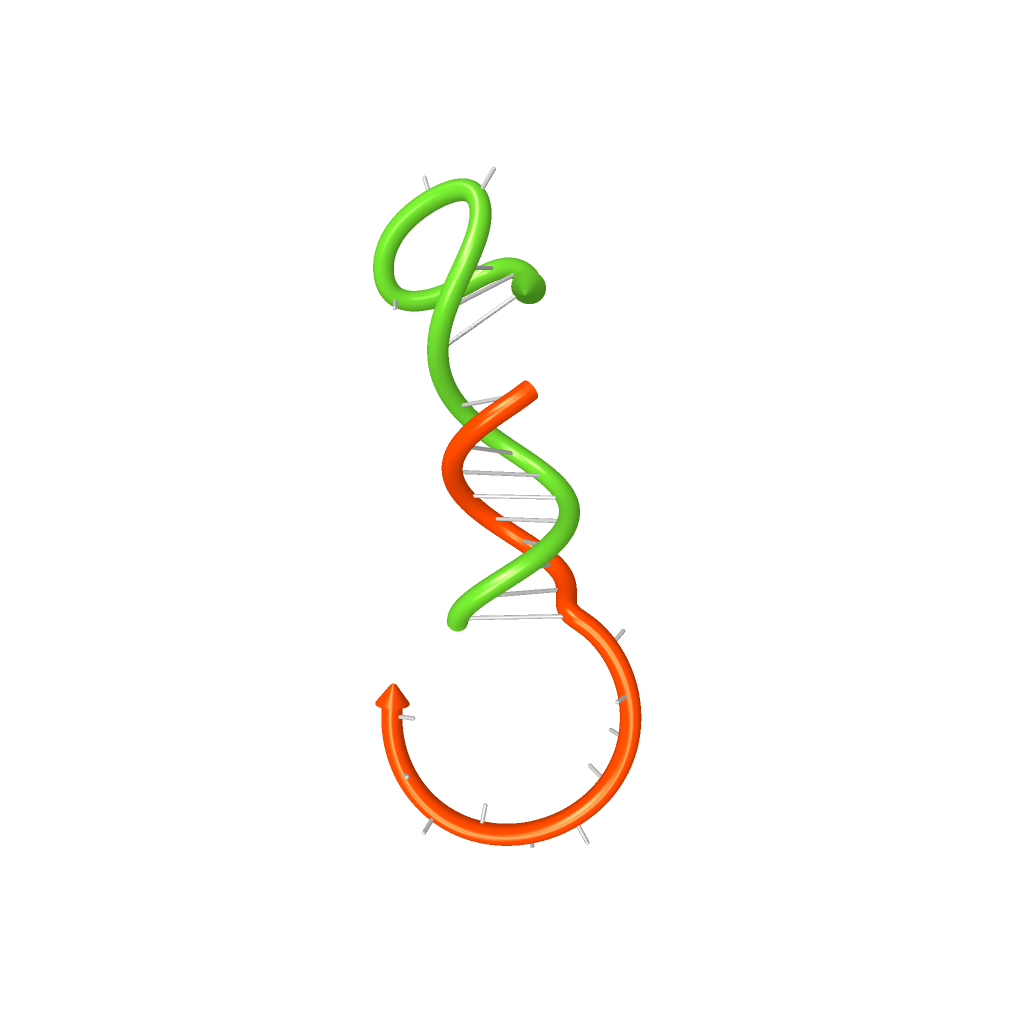
\includegraphics[width=2cm]{3DFamilies/H/1618555267_25d.png}};
\node[inner sep=0, right=0mm of H1] (H2) {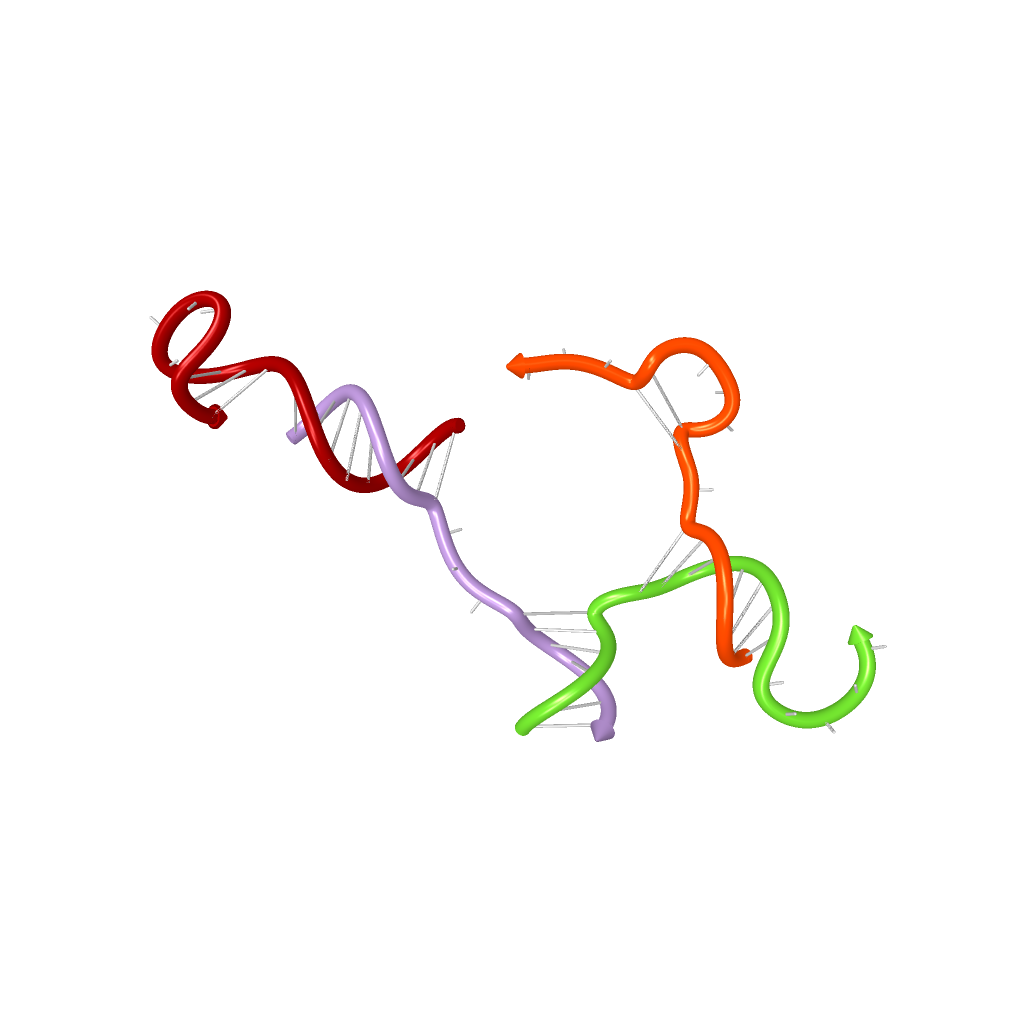
\includegraphics[width=2cm]{3DFamilies/H/1618555331_25d.png}};
\node[inner sep=0, right=0mm of H2] (H3) {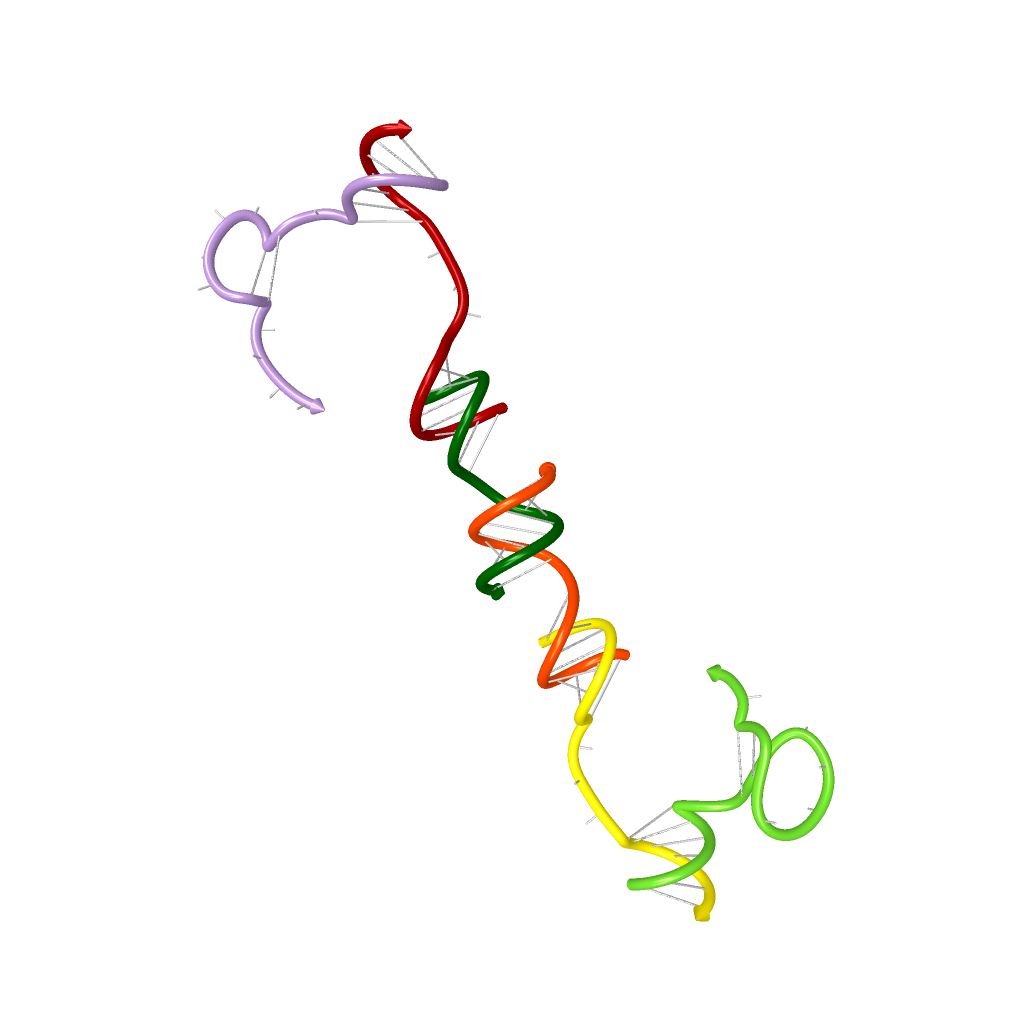
\includegraphics[width=2cm]{3d/L2-H_random.png}};


%%%%% L3 %%%%%

% I
\node[inner sep=0, below=5mm of G1] (I1) {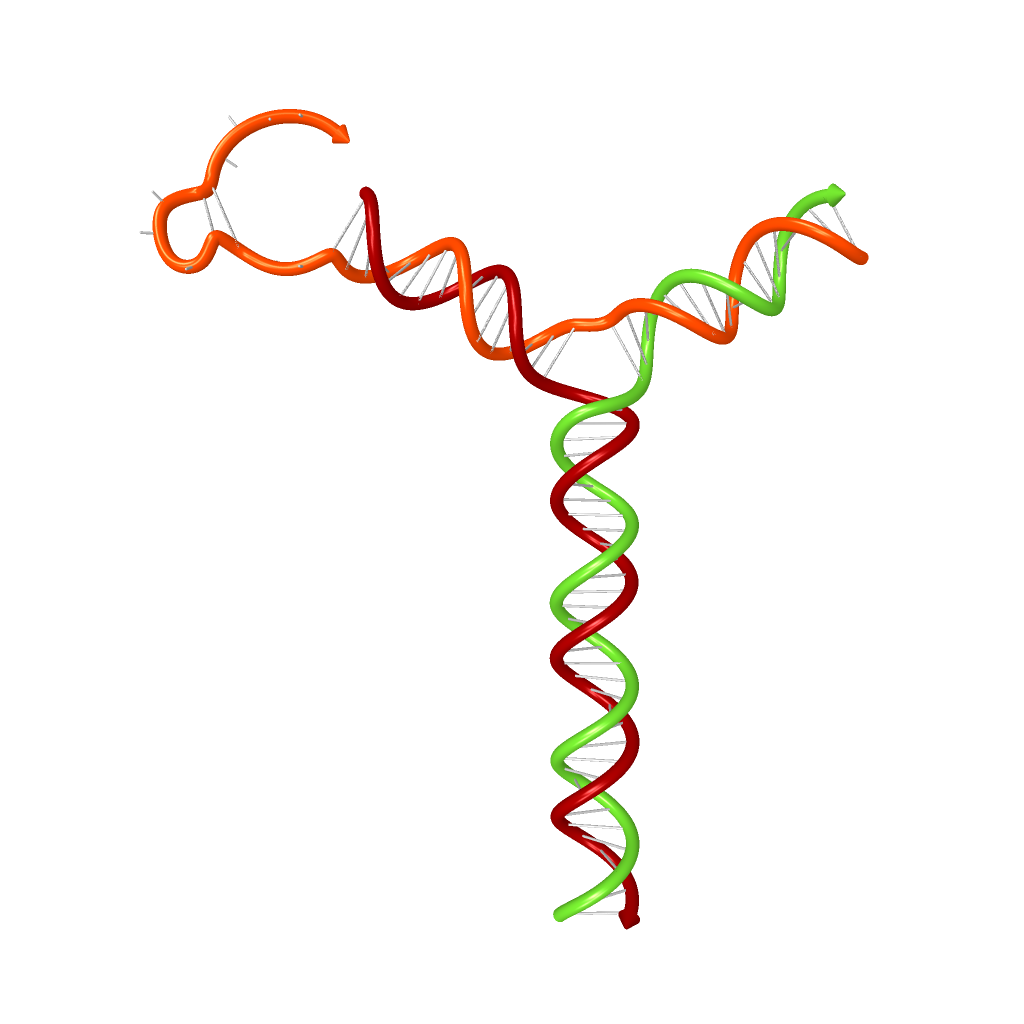
\includegraphics[width=2cm]{3DFamilies/I/1618729914_25d.png}};
\node[inner sep=0, right=0mm of I1] (I2) {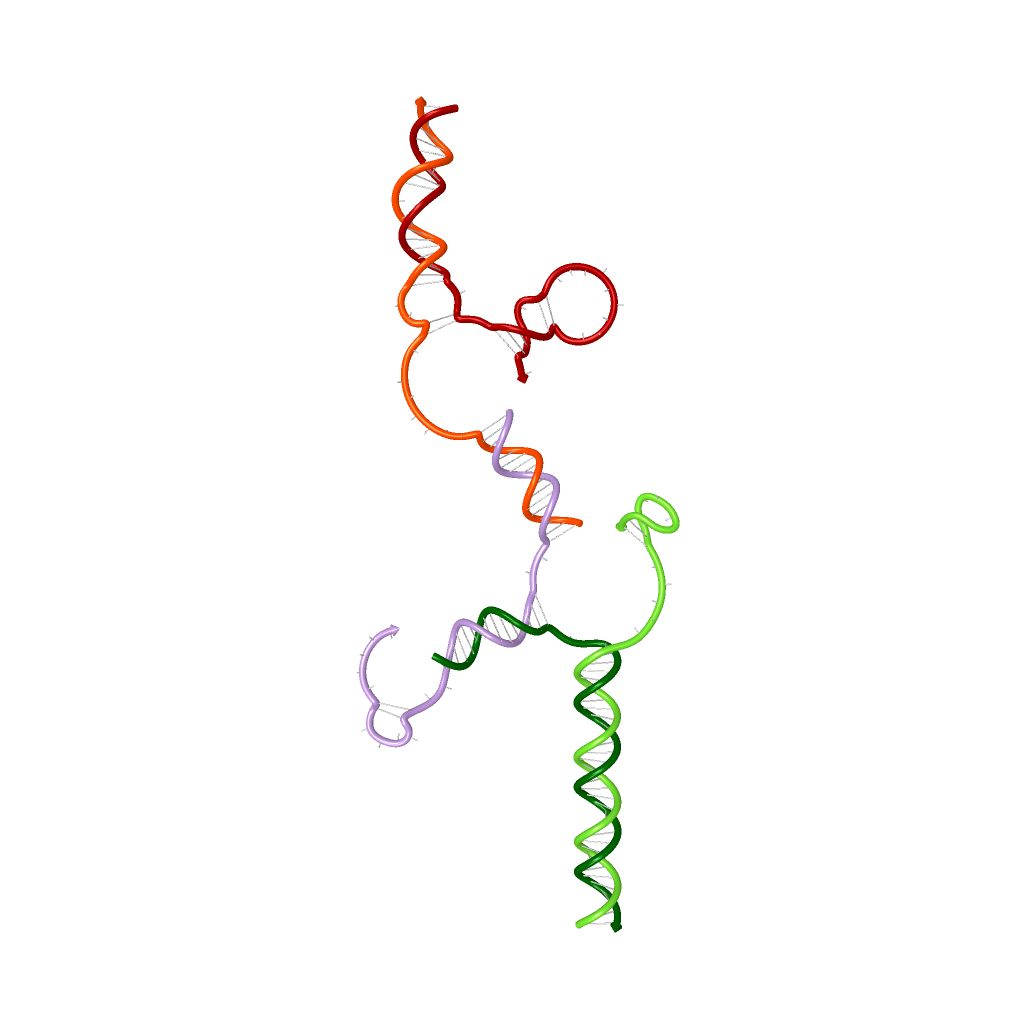
\includegraphics[width=2cm]{3DFamilies/I/1618730277_25d.png}};
\node[inner sep=0, right=0mm of I2] (I3) {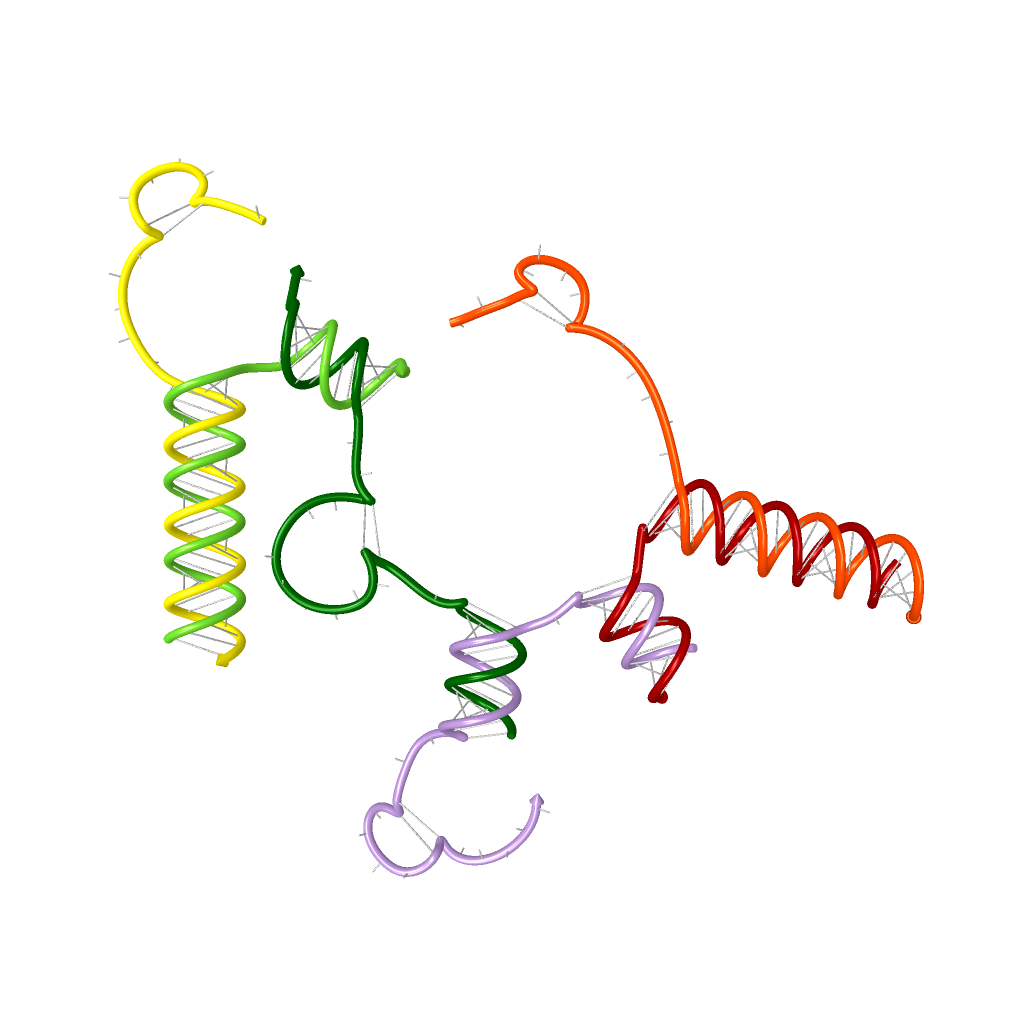
\includegraphics[width=2cm]{3d/L3-I_random.png}};

% J
\node[inner sep=0, right=10mm of I3] (J1) {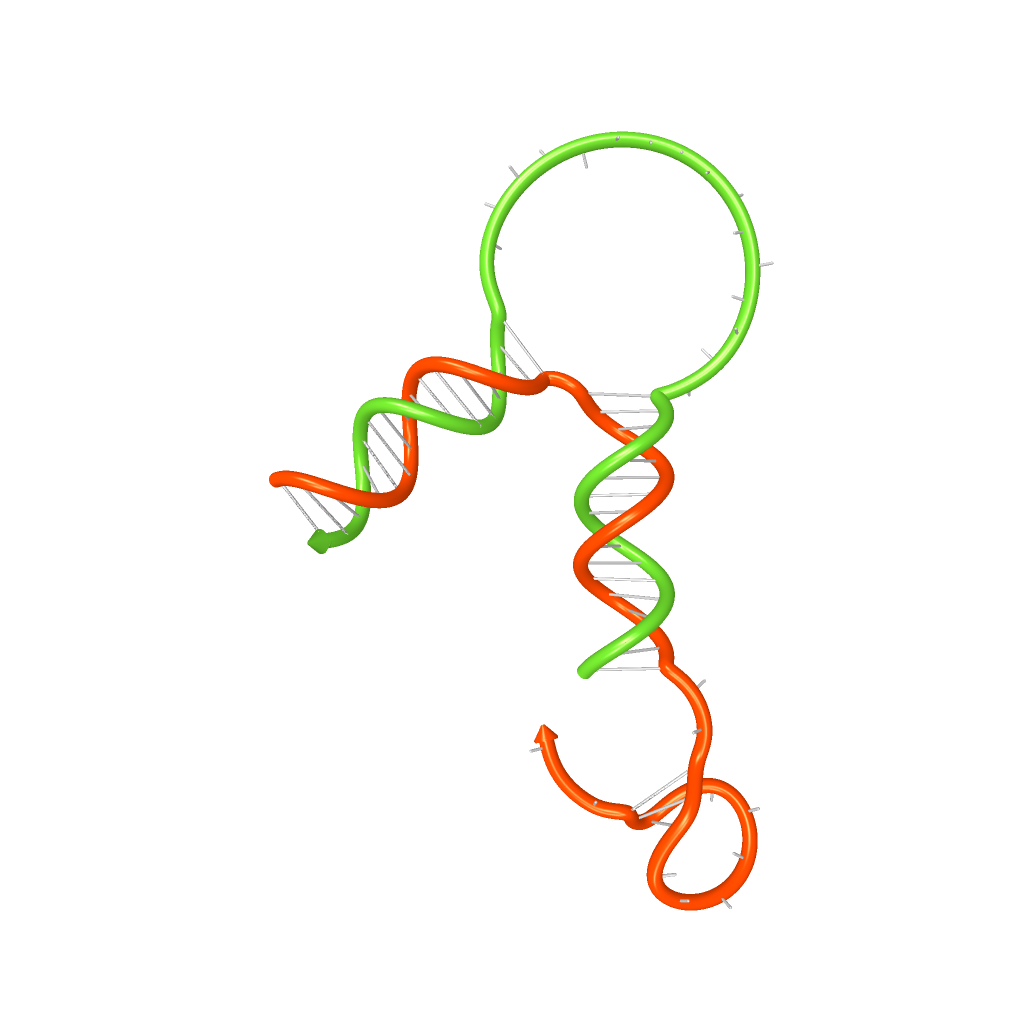
\includegraphics[width=2cm]{3DFamilies/J/1618791576_25d.png}};
\node[inner sep=0, right=0mm of J1] (J2) {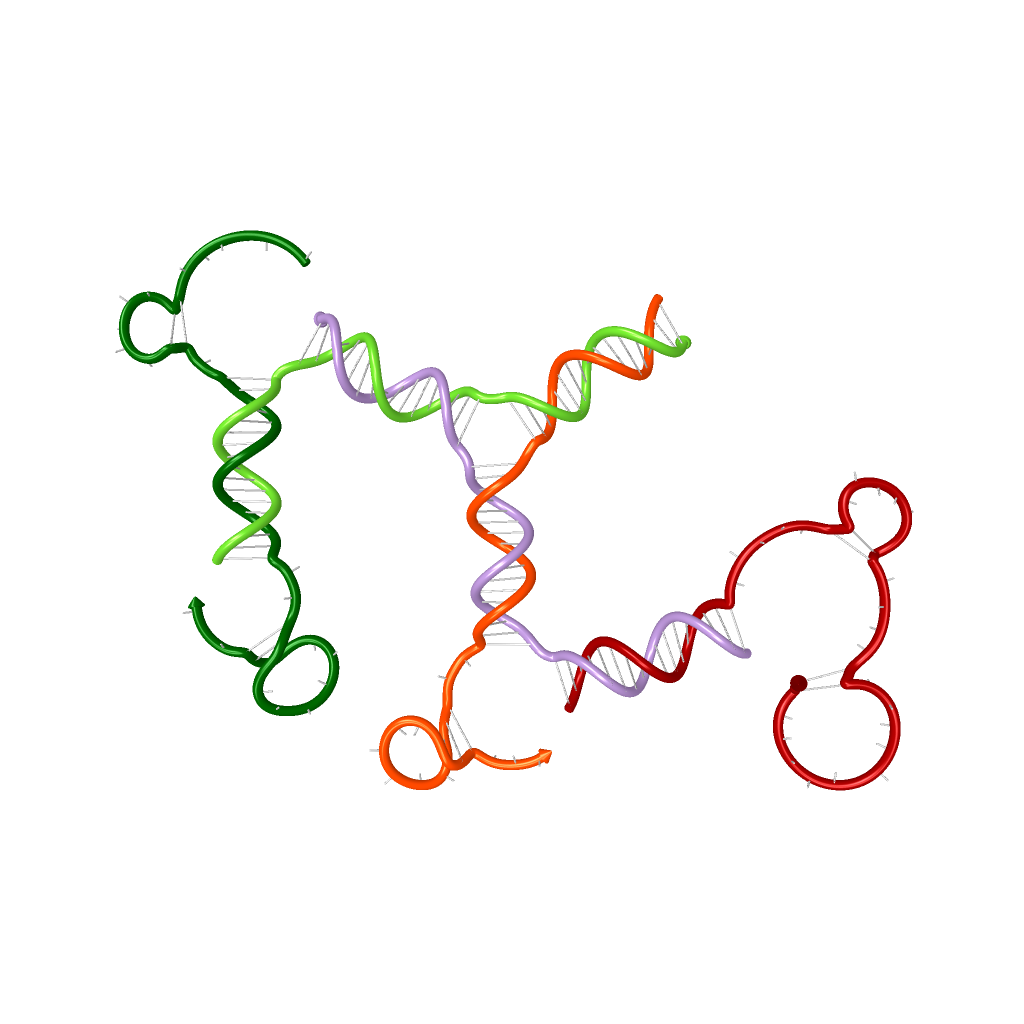
\includegraphics[width=2cm]{3DFamilies/J/1618791914_25d.png}};
\node[inner sep=0, right=0mm of J2] (J3) {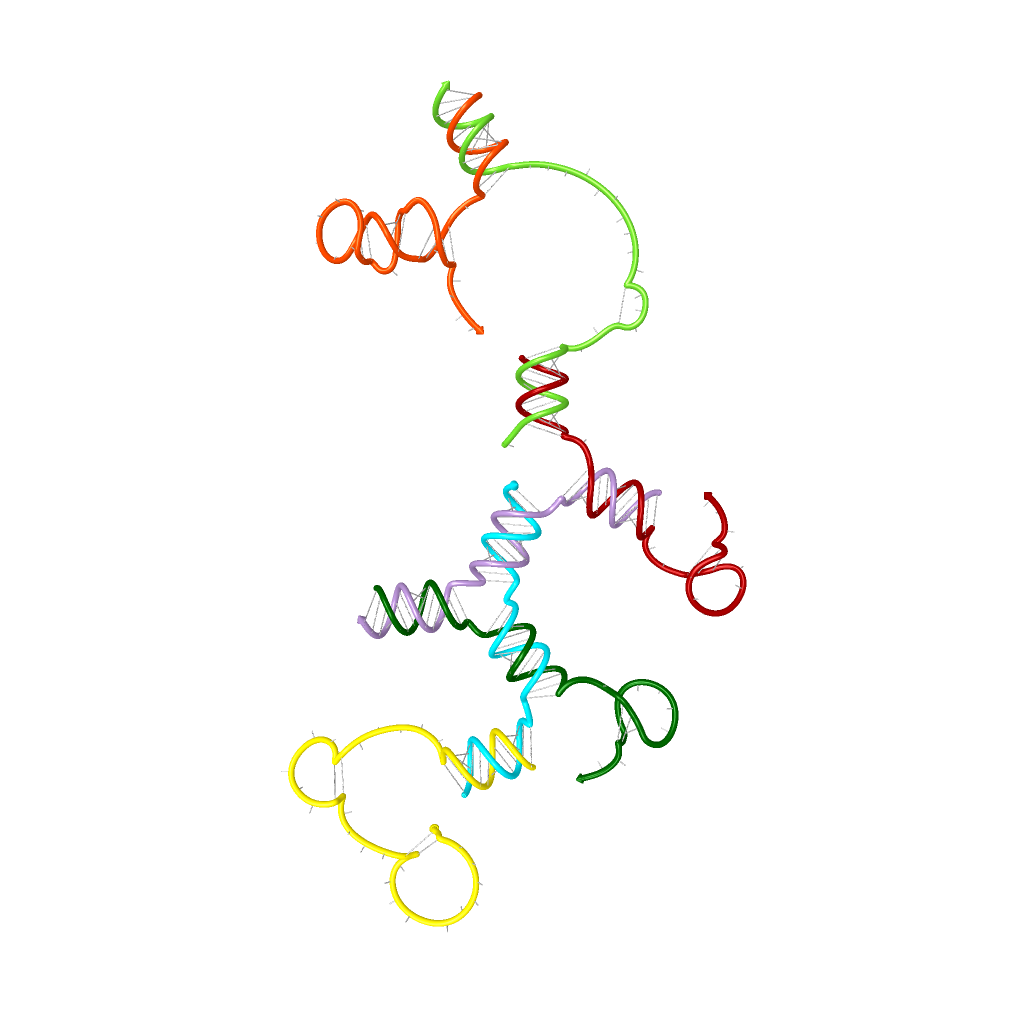
\includegraphics[width=2cm]{3d/L3-J_random.png}};

% K
\node[inner sep=0, below=0mm of I1] (K1) {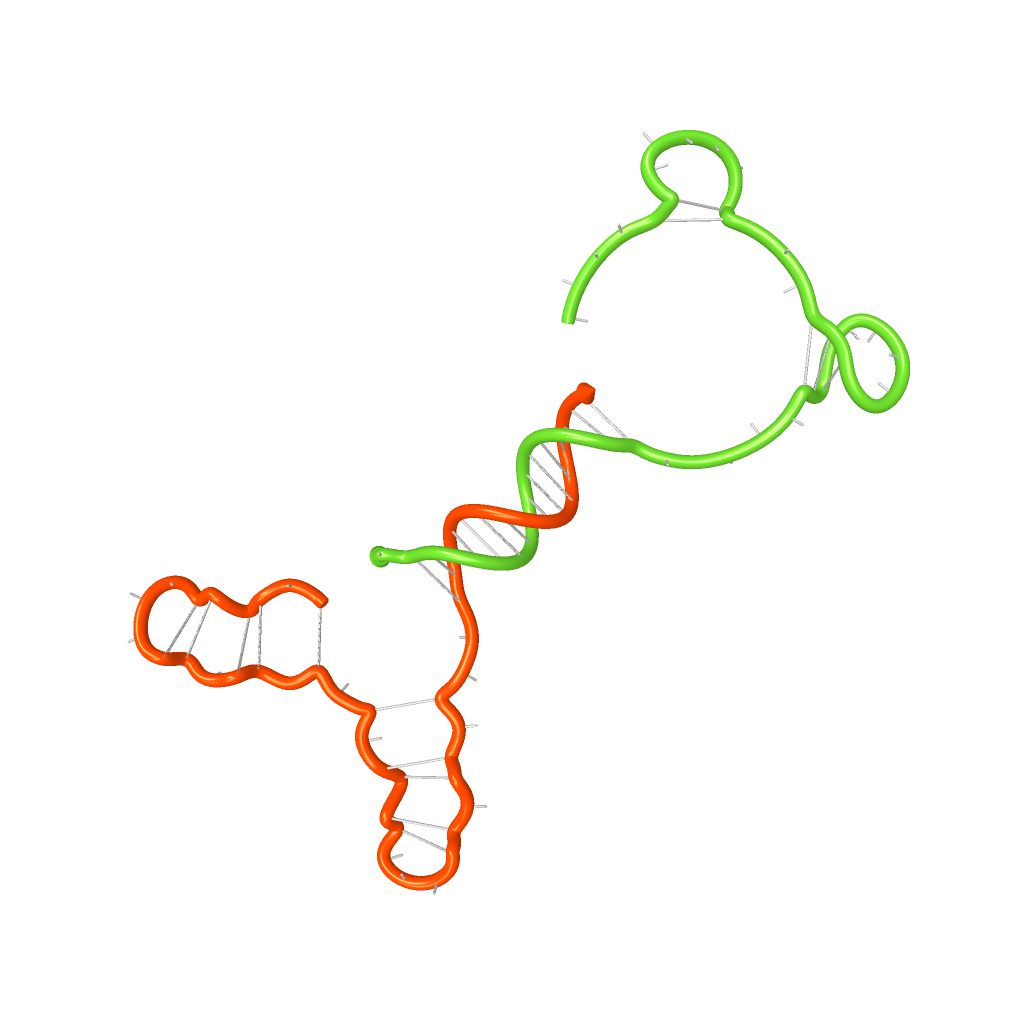
\includegraphics[width=2cm]{3DFamilies/K/1618793415_25d.png}};
\node[inner sep=0, right=0mm of K1] (K2) {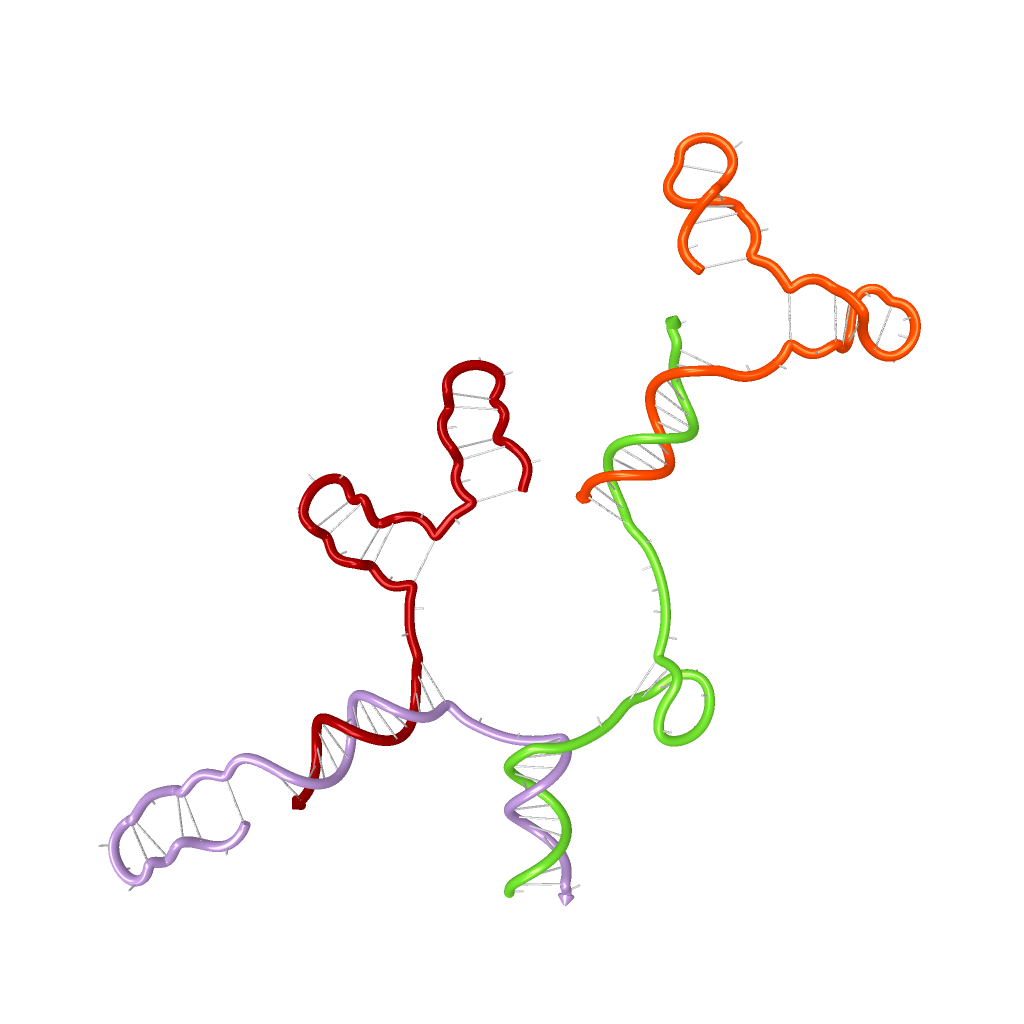
\includegraphics[width=2cm]{3DFamilies/K/1618793447_25d.png}};
\node[inner sep=0, right=0mm of K2] (K3) {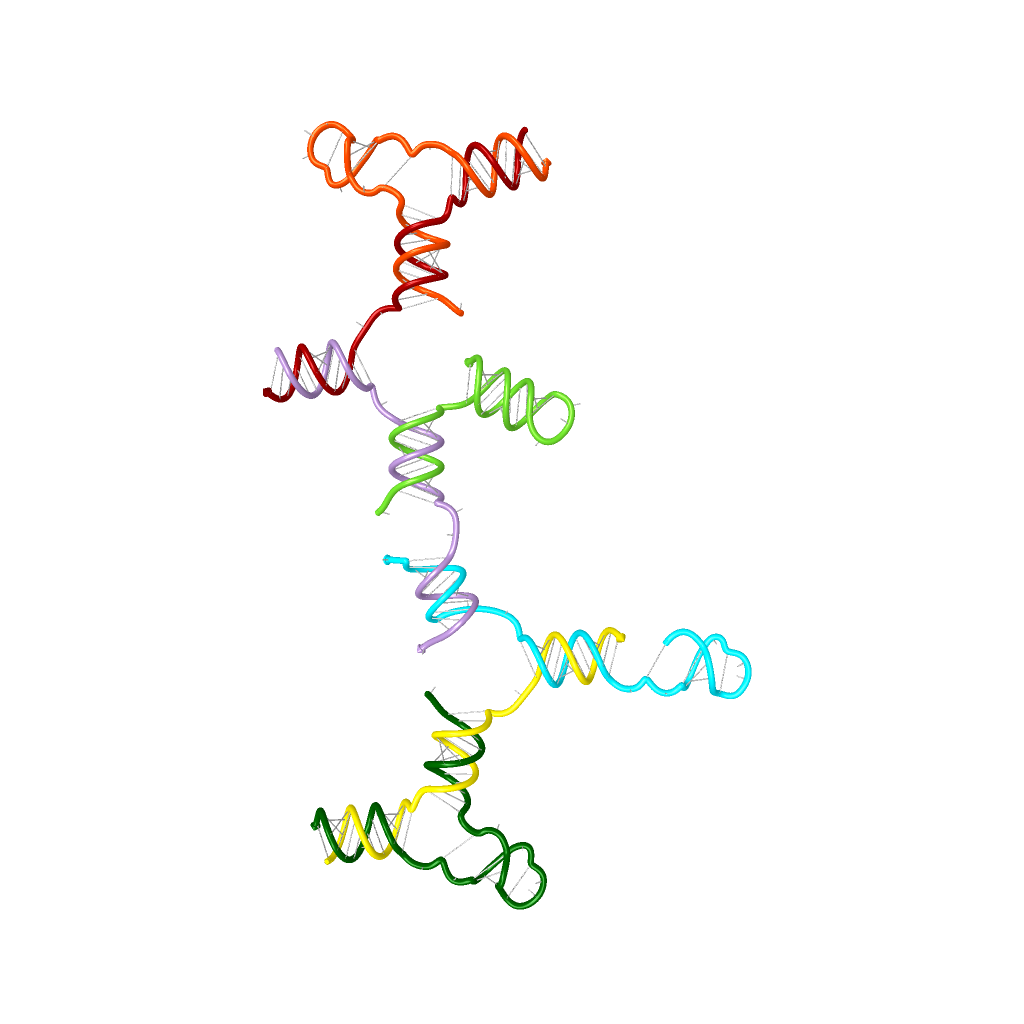
\includegraphics[width=2cm]{3d/L3-K_random.png}};

% L
\node[inner sep=0, right=10mm of K3] (L1) {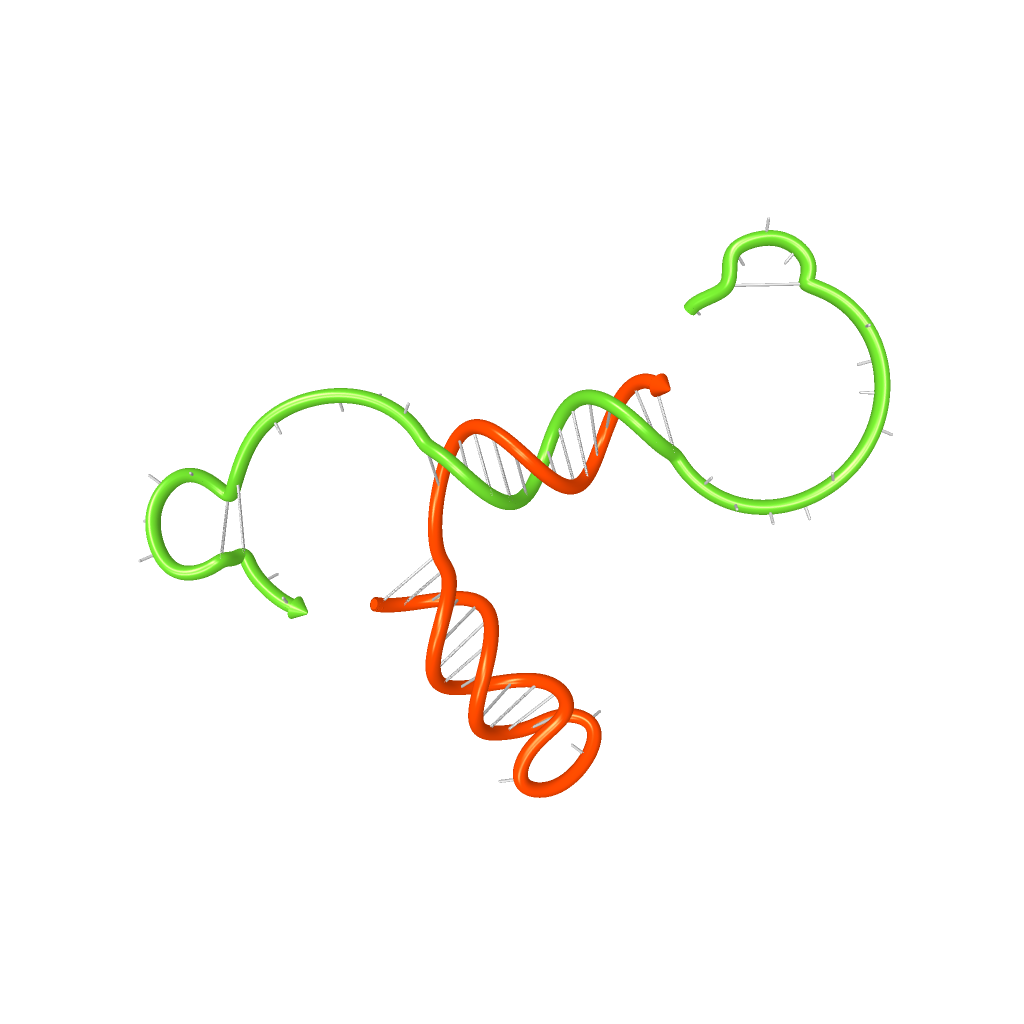
\includegraphics[width=2cm]{3DFamilies/L/1618458911_25d.png}};
\node[inner sep=0, right=0mm of L1] (L2) {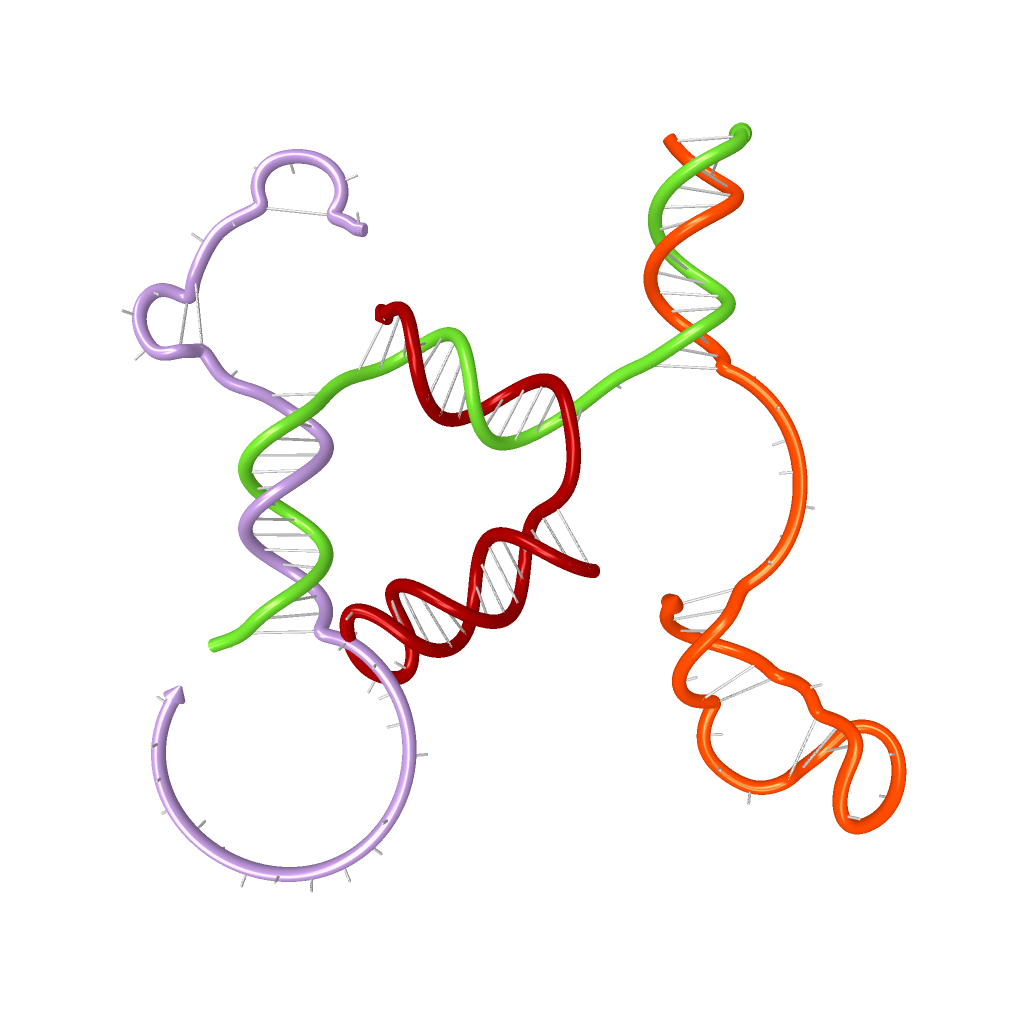
\includegraphics[width=2cm]{3DFamilies/L/1618458953_25d.png}};
\node[inner sep=0, right=0mm of L2] (L3) {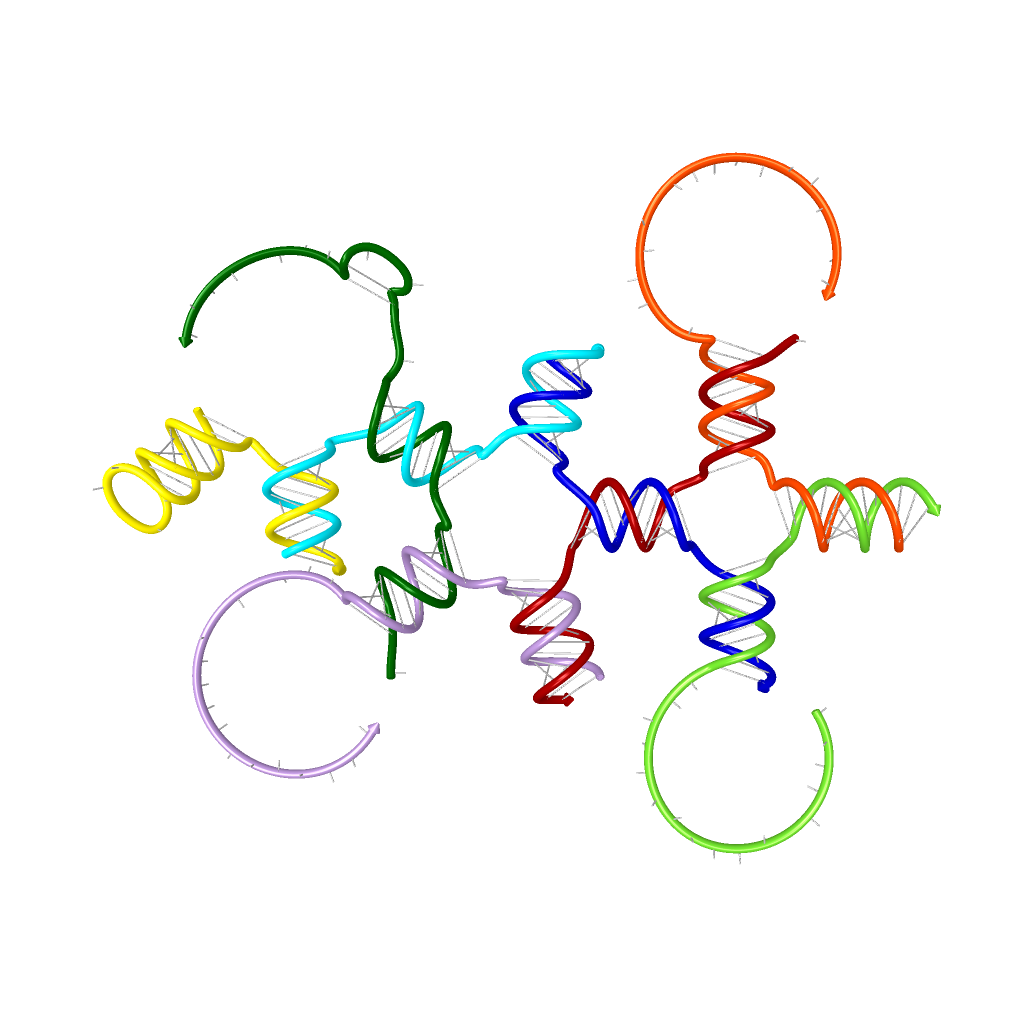
\includegraphics[width=2cm]{3d/L3-L_GA.png}};


% Titles
\node[color=black,left=0.5mm of A1,rotate=0,anchor=north,align=center,shift={(0.00,0.00)}] {A};
\node[color=black,left=0.5mm of B1,rotate=0,anchor=north,align=center,shift={(0.00,0.00)}] {B};
\node[color=black,left=0.5mm of C1,rotate=0,anchor=north,align=center,shift={(0.00,0.00)}] {C};
\node[color=black,left=0.5mm of D1,rotate=0,anchor=north,align=center,shift={(0.00,0.00)}] {D};
\node[color=black,left=0.5mm of E1,rotate=0,anchor=north,align=center,shift={(0.00,0.00)}] {E};
\node[color=black,left=0.5mm of F1,rotate=0,anchor=north,align=center,shift={(0.00,0.00)}] {F};
\node[color=black,left=0.5mm of G1,rotate=0,anchor=north,align=center,shift={(0.00,0.00)}] {G};
\node[color=black,left=0.5mm of H1,rotate=0,anchor=north,align=center,shift={(0.00,0.00)}] {H};
\node[color=black,left=0.5mm of I1,rotate=0,anchor=north,align=center,shift={(0.00,0.00)}] {I};
\node[color=black,left=0.5mm of J1,rotate=0,anchor=north,align=center,shift={(0.00,0.00)}] {J};
\node[color=black,left=0.5mm of K1,rotate=0,anchor=north,align=center,shift={(0.00,0.00)}] {K};
\node[color=black,left=0.5mm of L1,rotate=0,anchor=north,align=center,shift={(0.00,0.00)}] {L};

\node[color=black,left=5mm of A1,rotate=0,anchor=north,align=center,shift={(0.00,-0.75)}] {\Large{L1}};
\node[color=black,left=5mm of E1,rotate=0,anchor=north,align=center,shift={(0.00,-0.75)}] {\Large{L2}};
\node[color=black,left=5mm of I1,rotate=0,anchor=north,align=center,shift={(0.00,-0.75)}] {\Large{L3}};

%\node[color=black,above=7mm of A2,rotate=0,anchor=north,align=center,shift={(0.00,0.00)}] {\Large{L1}};
%\node[color=black,above=7mm of E2,rotate=0,anchor=north,align=center,shift={(0.00,0.00)}] {\Large{L2}};
%\node[color=black,above=7mm of I2,rotate=0,anchor=north,align=center,shift={(0.00,0.00)}] {\Large{L3}};


\end{tikzpicture}

\end{document}
